\vspace*{\fill}
In this part, we exhibit the three main contributions of our work.
First, we introduce SimRa, which is a mobile application for gathering cycling trip data and we also focus on our approach to automatically detect incidents in bicycle traffic in \cref{cha:cyclesense}.
Second, we suggest an approach to derive the road surface quality from cycling trip data and use the data gathered with SimRa to demonstrate how it works in \cref{cha:cyclequality}.
Third, we show our approach to improve the bicycle simulation of an urban traffic simulation software called SUMO, by utilizing the SimRa dataset to extract the lateral movement and the left-turn behavior of cyclists at intersections in \cref{cha:sumo}.
\vspace*{\fill}
\chapter{Gathering Cycling Trip Data and Detecting Incidents}
\label{cha:cyclesense}
In this chapter, we present SimRa\footnote{SimRa is an acronym for \textbf{S}icherheit \textbf{im} \textbf{Ra}dverkehr, which translates to safety in bicycle traffic from German.}, which is a crowdsourcing (see \cref{sec:crowdsourcing_crowdsensing_background}) platform for gathering cycling trip data.
A special feature of SimRa is it's capability to automatically detect incidents in bicycle traffic, which we also show in this chapter.
SimRa's main objective is to find out hazardous hotspots in bicycle traffic.
For this, we need to gather recordings of cycling trips, which have to contain user-generated information regarding the incidents, as well as a GPS trace, so that we can map the incidents and find out where they accumulate.

However, a cycling trip can be very long, both in distance and time, which complicates this process for the SimRa users since it can be difficult to remember every incident, its details and exact location.
While automatically recording the GPS trace during a cycling trip via a smartphone app is trivial, automatically gathering detailed information such as exact location, type and other participants of the incidents is not.
It is however possible for the SimRa app to make educated guesses \textit{where} an incident might have happened during a ride based on the data produced by the \ac{imu}, which provides us information about acceleration, orientation and other gravitational forces.
With this information, the user only has to remember whether an incident really happened there and what kind of incident it was, which makes their task easier.
For this, SimRa has two different mechanisms.
The first mechanism relies only on the \ac{imu} readings of the ride to suggest points in the ride where an incident might have happened and was available since the initial release of SimRa.
The second mechanism relies on a \ac{dl} model which was trained with labeled data and is better at detecting incidents, which eases the task of the SimRa users to provide all incidents together with their details.

This chapter combines material published in \cite{karakaya2020simra,karakaya2022cyclesense} and has following contributions:
\begin{itemize}
\item We describe the design of the SimRa platform, a crowdsourcing-based data collection and processing platform for cyclist routes and incidents.
\item We propose an approach that combines signal processing and \ac{ml} techniques to detect incidents based on motion sensor data of cyclists with an \ac{auc} \ac{roc} of 0.906.
\item We evaluate our approach using the SimRa data set and compare it to two baselines as well as common \acl{dl} models used in the context of \acl{tsc}.
\item We discuss to which degree our approach can automate incident detection and which additional sensors are needed for full automation.
\end{itemize}

This chapter continues with background information about \ac{dl} and \ac{tsc} following Ismail Fawaz et al.~\cite{ismail2019deep} in \cref{sec:deep_learning_background}, which is important to understand the second mechanism to automatically detect incidents, mentioned above.
Afterwards, we give a more detailed description about the SimRa mobile application in \cref{sec:simra}.
In \cref{sec:detecting_near_miss_incidents}, we explain how we use \ac{dl} to automatically detect incidents.
We evaluate our approach in \cref{sec:evaluation_cyclesense}, which we follow up with a discussion in \cref{sec:discussion_cyclesense}.
Finally, we give an overview of alternative approaches and summarize this chapter in \cref{sec:related_work_cyclesense} and \cref{sec:summary_cyclesense} respectively.

\section{Deep Learning for Time Series Classification}
\label{sec:deep_learning_background}
In this section, we explain background information about time series classification and deep learning, which is used by SimRa to automatically detect the incidents.

\subsection{Time Series Classification}
As we will see in \cref{sec:simra}, the SimRa dataset consists of multivariate time series.
A multivariate time series consists of $n \in \mathbb{N}$ different univariate time series $X_{i} \in \mathbb{R}_{t}$ with univariate time series $X = x_{1}, x_{2},...,x_{t}$ with each $x_{i} \in \mathbb{R}$ being chronologically ordered by $t \in \mathbb{N}$.
In short, a multivariate time series is a chronologically ordered set of variables, in our case different \ac{imu} readings.
An example of a univariate time series is the data produced by a distance sensor, where we have pairs of $(distance,timestamp)$, chronologically ordered by $timestamp$.
An example of a multivariate time series is a weather station database, that reports the temperature, humidity and wind force every hour.
The task of \ac{tsc} is to assign a one-hot label to each entry of the time series, e.g., whether the weather is safe for an airplane to fly or not. 

\subsection{Deep Learning for Time Series Classification}
With their rise, \acp{dnn} have drawn attraction to themselves from the field of \ac{tsc}.

\begin{figure}
    \center
    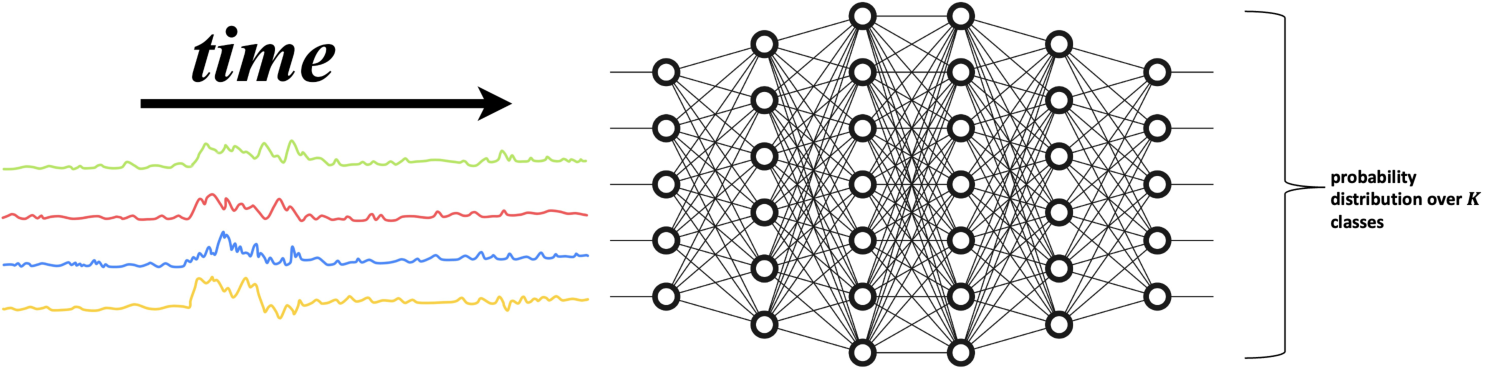
\includegraphics[width=\columnwidth]{fig/deep_learning_structure.pdf}
    \caption{Structure of a Deep Learning approach to time series classification: A classifier that maps a time series to a probability distribution of classes\cite{chen2021deep}}
    \label{fig:deep_learning_structure}
\end{figure}

As shown in figure~\ref{fig:deep_learning_structure}, a Deep Learning approach to \ac{tsc} consists of a classifier (in this case a \ac{mlp}, which is a type of a \ac{dnn}), that maps a time series to a probability distribution of $K$ classes.

\begin{figure}
    \center
    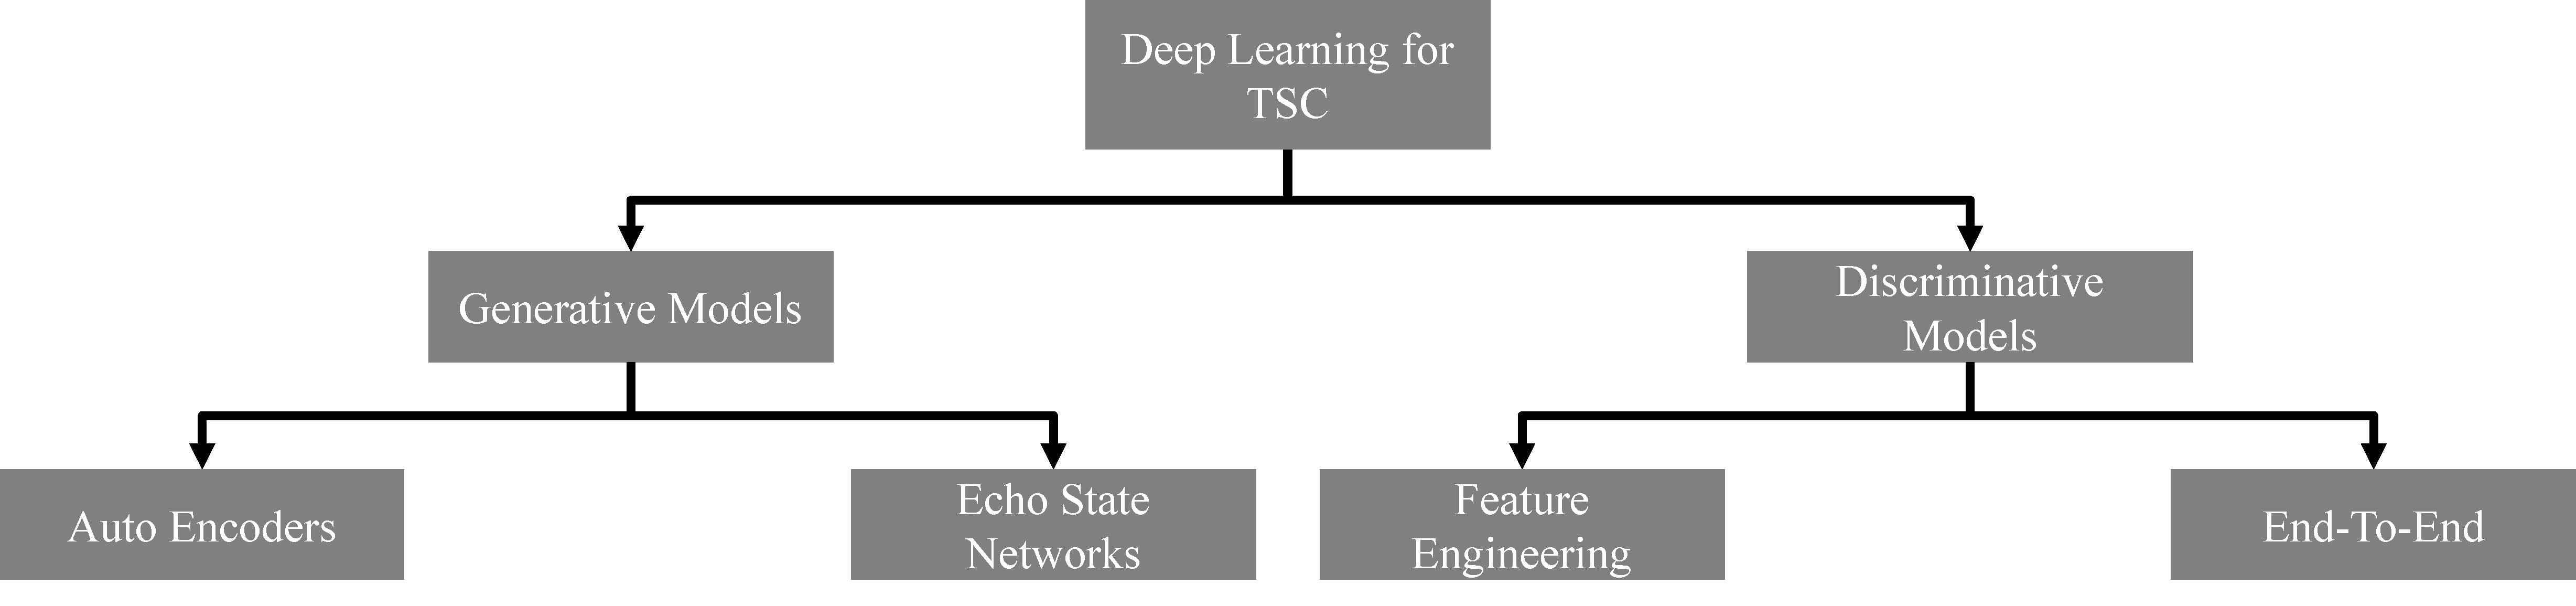
\includegraphics[width=\columnwidth]{fig/deep_learning_approaches.pdf}
    \caption{Taxonomy of Deep Learning approaches for Time Series Classification (based on L\"ankvist et al. and Ismail Fawaz et al.~\cite{langkvist2014review,ismail2019deep}}
    \label{fig:deep_learning_approaches}
\end{figure}

Figure~\ref{fig:deep_learning_approaches} shows the two categories of \ac{dl} approaches for \ac{tsc}, which were differentiated by L\"ankvist et al. and then extended by Ismail Fawaz et al.~\cite{langkvist2014review,ismail2019deep}.

\subsubsection*{Generative Models}
Generally, generative Models provide a probability distribution $P(x,y)$ with $x$ being the input data and $y$ being the label.
The label $y$ is determined by using the Bayes rules to calculate $P(y|x)$~\cite{ng2001discriminative}.
A generative model for \ac{tsc} usually consists of two parts~\cite{langkvist2014review}: First, a model of the dataset is derived with an unsupervised learning phase.
This model is then used to train a classifier that can successfully determine the correct label for each input.
Ismail Fawaz et al. classifies two different categories of Generative Models: \textit{Auto Encoders} and \textit{Echo State Networks}~\cite{ismail2019deep}.

\textit{Auto Encoders}, such as Stacked Denoising Auto-Encoders~\cite{bengio2013generalized}, \acp{cnn}~\cite{song2020representation}, Deep Belief Networks~\cite{banerjee2019deep}, \acp{rnn}~\cite{rajan2018generative}, split the the unsupervised learning preprocessing
and the training of the classifier.

\textit{Echo State Networks} on the other hand combine these steps~\cite{jaeger2001echo} to first reconstruct the dataset, to use the learned representation of it from the reservoir space~\cite{aswolinskiy2018time,bianchi2020reservoir,chouikhi2018genesis,ma2016functional}

\subsubsection*{Distinctive Models}
As stated by Vapnik~\cite{vapnik1998statistical}, the classification problem should be solved directly, without trying to solve a more general problem as an intermediate step.
This is what Distinctive Models do, and instead of first calculating $P(x,y)$, they derive $P(y|x)$, or a mapping from an input to the label directly~\cite{ng2001discriminative}.
Distinctive Models can be further categorized into \textit{Feature Engineering} and \textit{End-to-End}~\cite{ismail2019deep}.

As the name suggests, in \textit{Feature Engineering} the focus lies in the hand-engineering of the features.
In the most common form, which was inspired from computer vision, the time series is first transformed into an image~\cite{wang2015encoding,hatami2018classification,tripathy2018use}, so that the features could be hand-engineered correctly.
This approach does not need any domain-specific knowledge.
If domain-specific knowledge is available, the feature extraction can be done without transforming the dataset into images and the features can directly be included in the classifier~\cite{uemura2018feasibility,ignatov2018real}.

Contrary, in \textit{End-to-End} Deep Learning the feature extraction is included in the process and does not have to be made manually~\cite{nweke2018deep}.
Distinctive Models of the \textit{End-to-End}-type have been realized with \acp{mlp}~\cite{wang2017time,geng2019cost}, \acp{cnn}~\cite{che2017boosting,ismail2018evaluating,liu2018time} and hybrid networks~\cite{lin2017gcrnn,serra2018towards}.


\section{SimRa - A Platform for Gathering Cycling Trips and Incidents in Bicycle Traffic}
\label{sec:simra}
In this section, we give a general overview of the SimRa platform which comprises all things related to the collection, storage, and analysis of crowdsourced cycling data which we will focus on in the following sections.

\subsection{Goal of the SimRa platform}
\label{subsec:simra}

For data acquisition we rely on an app installed on the smartphones of participating cyclists.
This app collects data and detects incidents during bicycle trips, lets users add comments or labels, and anonymizes the data before uploading it to our servers (see \cref{subsec:data_acquisition}).
The anonymized data comprises information on cyclist routes, incidents, user demographics, as well as some aggregated trip statistics.
Finally, we continuously process and analyze collected data to gain insights into dangerous street segments and intersections.
For this, we have developed one approach for interactive exploratory data analysis based on a web application and one for confirmatory data analysis~\cite{bermbach2017cloud} which automatically derives a ``dangerousness'' score per street segment and intersection~\footnote{\url{https://simra-project.github.io/dashboard/}}.

\subsection{Data Acquisition}
\label{subsec:data_acquisition}
For data acquisition, we could either rely on dedicated hardware or use commonly available hardware such as smartphones.
While dedicated hardware has certain benefits, e.g., higher measurement precision, such projects are inherently limited in scale:
\begin{figure}
    \center
    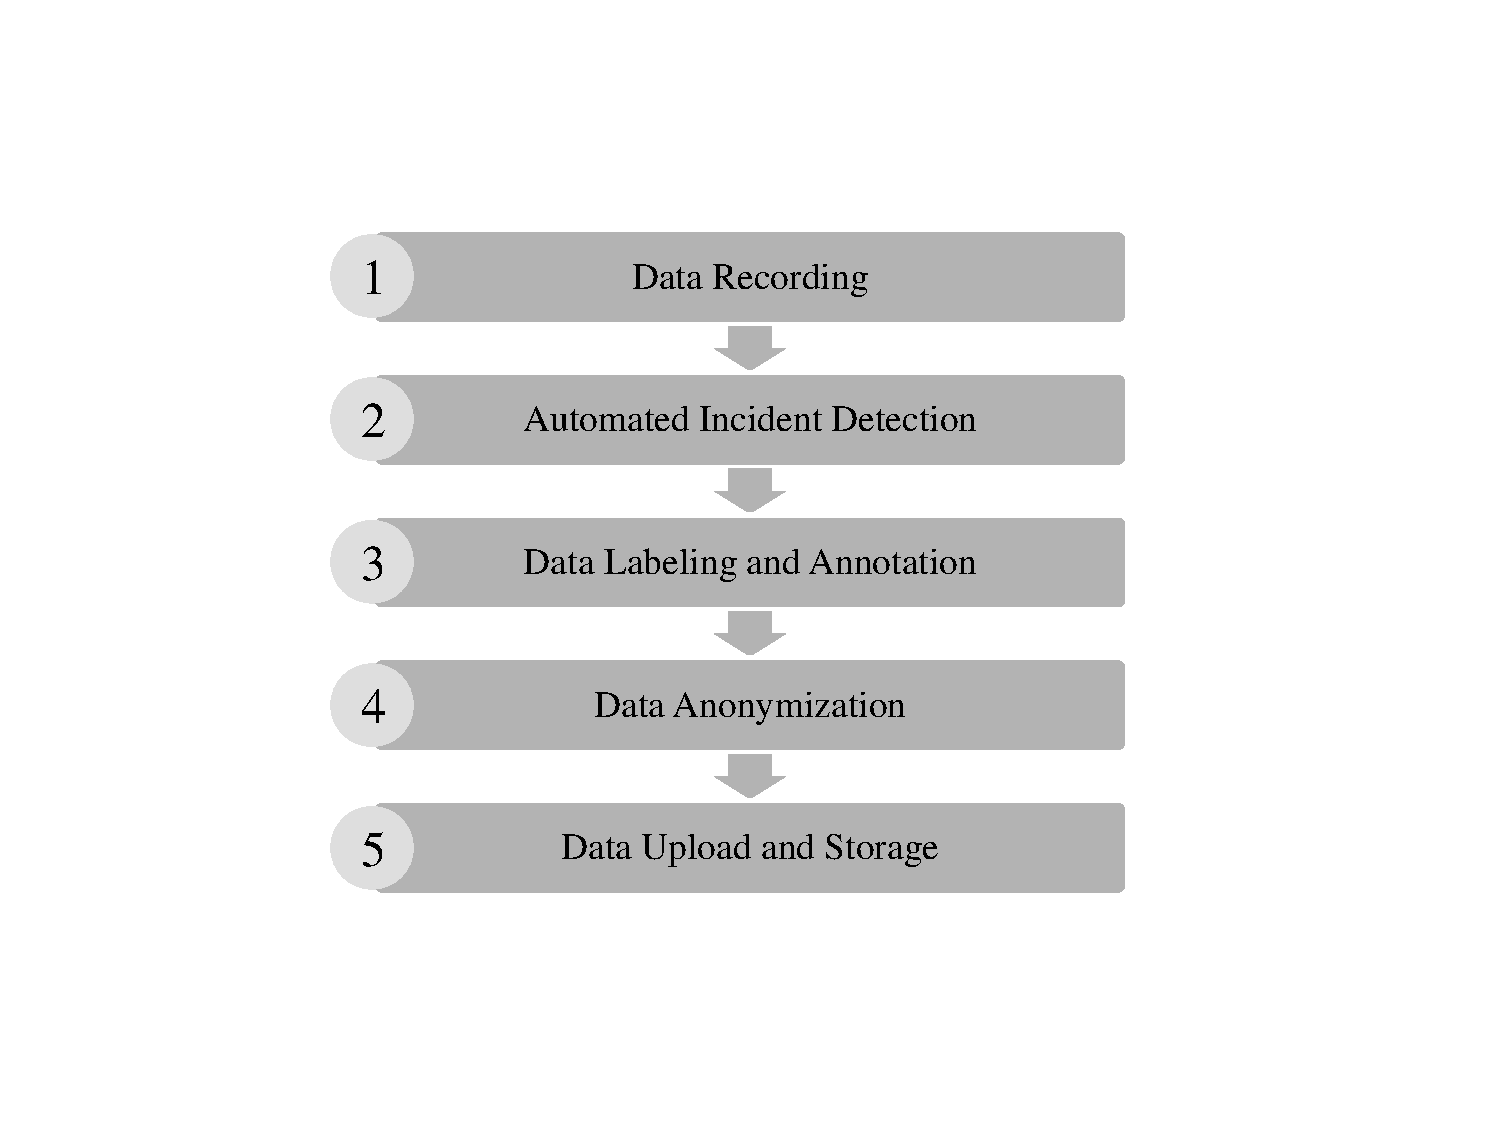
\includegraphics[width=0.5\columnwidth]{fig/data_acquisition_process.pdf}
    \caption{In the data acquisition process, collected data is manually annotated and anonymized before being uploaded to our backend servers.}
    \label{fig:data_acquisition_process}
\end{figure}
An example of this is the Radmesser project~\footnote{\url{https://interaktiv.tagesspiegel.de/radmesser/}} which built custom sensors to track close pass incidents.
While the data quality is indeed rather high, the project was limited to a total of 100 cyclists (only partly in parallel).
As a result, the project could not achieve full coverage of Berlin streets.
For example, some incident hotspots in terms of close passes that we were able to identify in SimRa did not even have a single bicyle trip in the Radmesser data.
We decided for project scalability and collect data with smartphones only.
Our goal is to collect data in a way that allows us (i) to identify incident hotspots as well as the kind of incidents and (ii) to identify the routes of cyclists (in which unnecessary detours are likely to identify severe incident hotspots).
%, and (iii) to collect additional data with the goal of improving automated incident detection.


Overall, our data acquisition process has five steps and follows the structure shown in figure~\ref{fig:data_acquisition_process} (we describe the steps in the following in detail).
This process runs continuously and in parallel as cyclists may create data for individual bicycle trips at any time.
During a trip, we first record sensor data using the built-in sensors of a cyclist's smartphone.
Upon completion of a trip, we analyze the raw data to automatically detect incidents.
Afterwards, the cyclist can enrich collected data with labels and annotations, use a number of anonymization measures, and upload the data to our backend servers.

\paragraph{Data Recording}
In the SimRa app, users manually start recording before they begin cycling (left part of Figure~\ref{fig:user-story}).
During a cycling trip, we track three sensors at varying rates per minute.
First, we query the GPS sensor every three seconds; this returns the current location and a radius with an accuracy confidence value of 68\%.
Second, we query the smartphone's accelerometer at 50Hz.
%These values include the effects of gravity and are in $m/s^2$.
While such a high sampling rate allows us to detect sudden peaks, this also leads to an unnecessary large data set which typically needs to be uploaded via mobile networks.
Thus, we aggregate the data based on a moving average across 30 values of which we only consider every sixth value.
This reduces the amount of data while still retaining all peaks in sensor readings.
Third, we store the device orientation based on the smartphone's gyroscope sensor every three seconds.
These values describe the rate of rotation around the X/Y/Z axis in rad/s and allow us to correctly interpret the direction of the acceleration values.
Each sensor measurement, together with a timestamp, is stored locally on the device.

We chose these rate settings based on initial experiments in which we identified the data collection rates and aggregation schemes as a sweet spot between system overload and information loss.



\paragraph{Automated Incident Detection}
After a cycling trip, as soon as the cyclist stops the recording, we analyze the recorded data to identify incidents.
The challenge, here, is to reliably detect incidents -- initially, without any training data.

For this reason, we developed a heuristic for incident detection that relies on the assumption that incidents will often materialize as sudden acceleration spikes.
After reaching over 10,000 labeled trips, we started to explore alternative detection methods ranging from machine learning to signals processing.
In our heuristic, we group the acceleration time series in three-second buckets to differentiate incidents and poor road conditions (e.g., potholes result in high vertical acceleration).
In each bucket, we identify the minimum and maximum value for every dimension and calculate the difference between those two.
In a second step, we categorize the six highest difference values across all buckets as likely incidents.
This allows us to separate high acceleration values based on poor road conditions (which usually have low difference values) from incident-related peaks.

In practice, this heuristic works well for cyclists with a ``relaxed'' cycling style.
For cyclists with a more ``rapid'' style of cycling, our heuristic usually identifies either accidents, severe bumps, or traffic lights but usually not incidents.
The heuristic is also inherently limited as it cannot detect close passes and similar incidents which do not materialize as acceleration spikes.

There was an alternative approach~\cite{sanchez2020detecting} using a simple Fully Connected Network (FCN) architecture without considering gyroscope sensor features yet.

\paragraph{Data Labeling and Annotation}

Even though we plan to improve the automated detection of incidents, some incident types cannot be automatically detected based on the sensor data alone.
For example, while being tailgated might make the cyclist increase speed, this kind of observable activity can also be related to other, non-dangerous events.
Thus, we do not think that a fully automated detection, also based on our hardware limitations, is a realistic option for SimRa -- neither now nor in the future.
Instead, we ask the cyclist to edit the pre-detected set of incidents (i.e., add false negatives and ignore false positives) and to label and annotate the correct set of incidents (right part of Figure~\ref{fig:user-story}).
%(see also section~\ref{sec:data} which describes the resulting data in detail).

\paragraph{Data Anonymization}

One of our side goals in SimRa is to preserve the privacy of our users, which is mainly achieved through three mechanisms: \emph{Delayed recording} allows users to define a time and a distance threshold after which a recording will start, \emph{trip cropping} allows users to crop their bicycle trip manually to hide where they started or arrived (middle part of Figure~\ref{fig:user-story}), and \emph{per-record pseudonymization} stores demographic and trip data separately so that they cannot be connected to individual users.
Furthermore, each trip is pseudonymized separately.

\paragraph{Data Upload and Storage}
Finally, and only when explicitly triggered by the cyclist, the cycling trip data is uploaded to our backend.
For authentication, we calculate an access key based on the current timestamp and a random salt which we update with new app versions.
This is necessary to avoid automated attacks on our backend as we do not have a notion of user accounts.
So far, this has sufficed as extracting the salt from the app binary requires enough manual effort to make this infeasible for automated attacks.
Note, that we store trips and user data per region so that we can analyze (geographic) regions separately.

\begin{figure}[ht]
	\centering
	\includegraphics[width=\textwidth]{fig/screenshots.png}
	\caption{Screenshots of the SimRa app depicting the user story from left to right.}
	\label{fig:user-story}
\end{figure}


\paragraph{Resulting Data}
The SimRa data set consists of more than 114,500 rides from over 100 regions.
Berlin accounts for the majority of rides of any region: Almost half the rides and incidents have been recorded there.
Hanover and Nuremberg are the next largest regions with approximately 8000 and 5500 rides respectively\footnote{65,000 rides from over 65 regions and 3500 rides for Hanover and Nuremberg each, when we submitted our paper~\cite{karakaya2022cyclesense}}.
The SimRa data set and source code are available online and in data repositories\footnote{https://github.com/simra-project/}.
Due to per ride pseudonymization, we used only ride data for our classifier and could not rely on profiles of individual cyclists.
Each ride file has two parts: The incident part and the ride part.
The incident part lists all incidents of the ride.
The ride part consists of timestamps, GPS, accelerometer, and gyroscope sensor readings. In more recent versions of the app, linear accelerometer and rotation vector data are also included.
The recording frequencies of the various sensors vary a lot (See table~\ref{tab:theoretical-measurements}) and as a result require a partition of the SimRa data set in three distinct parts: older Android rides, newer Android rides, and iOS rides.



\begin{table}[ht]
	\centering
	\resizebox{1.0\columnwidth}{!}{%
	\begin{tabular}{cccccc}
		\hline
		& \textbf{Accelerometer} & \textbf{Gyroscope} & \textbf{\ac{gps}} & \textbf{Linear accelerometer} & \textbf{Rotation vector} \\
		\hline\hline
		\textbf{Android old} & 10 Hz & 0.33 Hz  & 0.33 Hz & \textbf{/} & \textbf{/} \\
		\hline
		\textbf{Android new} & 4 Hz & 4 Hz  & 0.33 Hz & 4 Hz & 4 Hz \\
		\hline
		\textbf{iOS} & 10 Hz & 0.33 Hz  & 0.33 Hz & \textbf{/} & \textbf{/} \\
		\hline
	\end{tabular}%
	}
	\caption{Theoretical measurement frequencies of different sensors in different parts of the SimRa data set. 
		Note that these are only the theoretical frequencies that deviate significantly from the empirical measurement frequencies that can be observed in the data set (see Section \ref{sec:discussion_cyclesense}).}
	\label{tab:theoretical-measurements}
\end{table}

\paragraph{Crowdsensing or Crowdsourcing?}
Neither of the terms crowdsensing and crowdsourcing (see \cref{sec:crowdsourcing_crowdsensing_background}) fit perfectly to SimRa.
While SimRa could be classified as a \textit{infrastructure application} with a \textit{mobile sensing} approach as \textit{data collection} in the context of crowdsensing, the participants have to contribute more than just the data from the \ac{imu}.
They are also asked to classify, annotate and describe the incidents they encounter during their cycling trip.
If we go through the different aspects that characterize a crowdsourcing application (see \cref{sec:crowdsourcing_crowdsensing_background}) we can say that SimRa is a light-weight crowdsourced application.
The \textit{degree of human involvment} is medium.
While the users have to start and stop the recording and have to give additional information about the ride and incidents, no input is needed during the cycling trip and the app records the trip passively.
There is rather higher degree of \textit{location relevance}.
Although the annotation of the ride can be done wherever, a cycling trip can only be recorded when the cyclist is physically at a location.
It is not possible to record a ride in a location without being physically there (at least not without spoofing the GPS location of the smartphone).
There is a minimal \textit{knowledge requirement} the participants have to fulfill.
They must know, that they only have to report incidents and not a static hazard or a nuisance such as a very long red light.
The \textit{participation incentive} in SimRa is purely intrinsic.
There are no external benefits in using SimRa, such as monetary compensation.
The \textit{data flow} is hybrid, since there is preprocessing involved in the SimRa app, that happens on the smartphone.
However, it would be wrong to label SimRa as a fully fledged crowdsourcing project, since the \textit{Application User} and \textit{Data Processing Platform}, are basically merged together and there is no allocation of tasks.
The task is to record cycling trips, add additional details about the trip and the incidents and upload the data.
Hence, we consider SimRa as a (lightweight) crowdsourcing project.

\paragraph{SimRa and Citizen Science}
SimRa can clearly be considered as a Citizen Science project, as it fulfills the Ten Principles of Citizen Science (see \cref{sec:citizen_science_background}):
\begin{enumerate}
\item The users are crucial for the project, as they contribute their cycling trip data.
\item There is a genuine science outcome, as this thesis shows and the informing management decisions and environmental policies.
\item While the benefits of the citizen scientists are not as apparent as the professional scientists, they also profit in the long run, if the project goal improving the bicycle traffic safety increases.
\item While the citizen scientists' main task is to contribute cycling trip and incident data, they are free and encouraged to also participate in other stages of the scientific process.
E.g., the dataset is published as open data and everyone can analyze the data for insights about traffic safety.
\item We provide multiple channels for the citizen scientists to inform themselves about the progress of the project, such as through our social media account\footnote{\url{https://twitter.com/SimRa_App}} as well as a website\footnote{\url{https://simra-project.github.io/}}.
\item In each of our published papers, as well as in this thesis, we point at possible limitations and biases (see \cref{sec:discussion_cyclesense,sec:discussion_cyclequality,sec:discussion_sumo,sec:limitations_of_crowdsourced_data}). 
\item We publish the SimRa dataset as open data~\cite{dataset_simra_set1,dataset_simra_set2,dataset_simra_set3}
\item While we don't mention any citizen scientists directly, since there would be too many, we make sure that it is obvious, that we rely on participating citizen scientists.
\item In each of our published papers, as well as in this thesis, we evaluate the scientific output (see \cref{sec:evaluation_cyclesense,sec:evaluation_cyclequality,sec:evaluation_sumo}). 
\item We designed SimRa to be as privacy friendly as possible and have a very strict privacy policy statement\footnote{https://www.tu.berlin/en/mcc/research/projects/simra-privacy-policy-statement}.
\end{enumerate}

\section{Detecting Incidents with Deep Learning}
\label{sec:detecting_near_miss_incidents}
This section describes the process of automatically detecting incidents. 
Please note that the SimRa data are not optimized for automated processing and \ac{ml} but rather for aggregated statistics and review by humans.
Therefore, several preprocessing steps are needed (Section~\ref{subsec:preprocessing}).
We describe our \ac{ml} model in Section~\ref{subsec:model_architecture} and the training process in Section~\ref{subsec:model_training}.


\subsection{Preprocessing}
\label{subsec:preprocessing}
To overcome some limitations of the SimRa data set, we use data cleaning and preprocessing steps, in a sequential multi-stage manner, some of which are specific to some model types that will be used afterwards to classify the incidents within bicycle trips.

Before the preprocessing phase, a typical trip can be expressed by a $n \times d$ sparse matrix $X^{(i)}$, where $d$ describes the number of sensor features and $n$ represents the number of timestamps in a given trip $i \in \{1,...,R\}$.

Note that we typically only use the accelerometer, gyroscope, and \ac{gps} sensor features.
Using the linear accelerometer features in addition did not lead to a significant improvement.
Furthermore, the linear accelerometer and the rotation vector features are only available in the newer Android trips.
The non-sensory features such as phone location and bike type have a non-logical strong correlation with incidents caused by issues in the data recording phase and are therefore not used.

\begin{figure}[t]
	\centering
	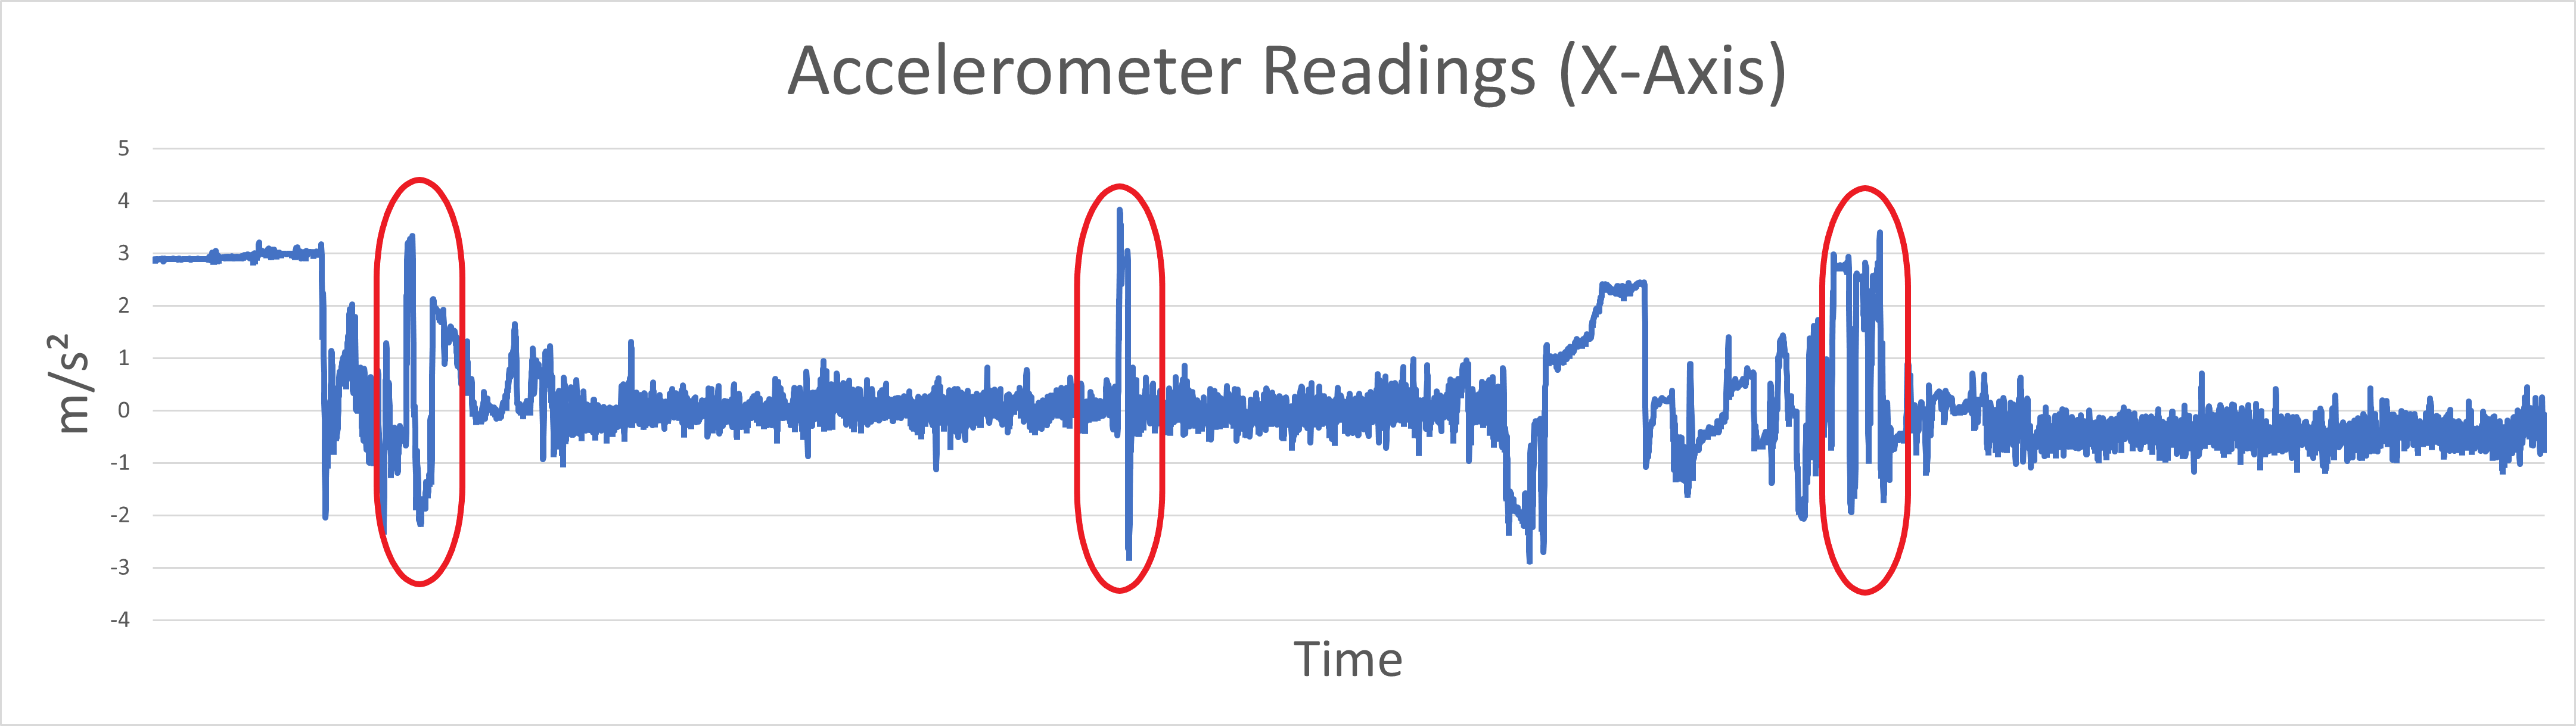
\includegraphics[width=0.5\textwidth]{fig/accelerometer-x-axis.png}
	\caption{The accelerometer readings of an example bicycle trip. The encircled spots could indicate an incident but also driving over a curb.}
	\label{fig:x-axis}
\end{figure}

The preprocessing pipeline starts off with a manual label cleaning procedure that aims to remove some of the wrongly labeled incidents.
Identifying them solely based on time series data is practically impossible for a human.
When visualizing the accelerometer sensor readings, incidents usually stand out as sudden spikes (see Figure~\ref{fig:x-axis}), but they also could be caused by driving over a curb or suddenly stopping due to a red light.
Therefore we focus on the incidents that feature an additional description that was provided by the users.
As it is very time-consuming, this is the only manual preprocessing step, and we apply it only to the newer Android data set.
Note that this procedure did not result in a fully cleaned data set.
Next, the timestamps within trips are sorted.
Afterwards, we sort out invalid rides, i.e., rides that contain adjacent timestamps that have been recorded with a gap of more than 6 seconds.
Furthermore, we remove outliers based on the statistical definition of outliers by Tukey et al.~\cite{tukey1977exploratory} that characterizes a data point as an outlier if it fulfills one of the equations $Outlier < q_{25} - k \cdot IQR$ or $Outlier > q_{75} + k \cdot IQR$ where the \ac{iqr} is equal to the difference between the upper and lower quartiles \cite{upton1996understanding, zwillinger1999crc}.
The $k$-values we are utilizing are 1.5 for \ac{gps} outliers regarding the accuracy feature and 3.0 for velocity outliers, as we have seen reasonable results for these values.

In a further step, speed is calculated from the distance between two \ac{gps} coordinates and their respective timestamp.
Moreover, the accelerometer and gyroscope sensor data are interpolated to create equidistance over the whole time series.
This is advisable, as unevenly spaced time series data tend to pose a problem to typical \ac{ml} solutions~\cite{weerakody2021review}.
Therefore, we up-sample to a frequency of 10 Hz via linear interpolation on uniformly generated timestamps with a 100 ms interval.
That means the up-sampling factor is usually above 2.
Although some argue that interpolation is a bad solution for unevenly spaced time series data in the context of \ac{tsc}~\cite{hayashi2005covariance, eckner2012framework}, initial experiments have shown that this improves model performance.
This preprocessing stage results in dense matrices $X^{(i)}$

For better convergence of the stochastic gradient descent optimizer used in the neural network, we normalize each feature individually by its maximum absolute value.
This is nearly always an advantageous preprocessing step as it improves model stability~\cite{bishop1995neural}.

Training the model on individually labeled timestamps did not appear to be a promising approach since incidents have a certain duration, which is typically longer than 100 ms, and it is highly unlikely that the user correctly specifies the label at the exact timestamp when the incident occurred.
For that reason, we split our ride data into 10-second buckets, following a non-overlapping sliding window approach~\cite{ortiz2011dynamic}.
These buckets are then labeled in the following manner: we define a bucket as an incident bucket if any timestamp inside that bucket was labeled as an incident.
Otherwise, we define it as a non-incident bucket.

Additionally, we apply a one-dimensional $f$-point \ac{dft} on each dimension of the accelerometer and the gyroscope sensor data contained in a bucket individually.
This results in a more advanced temporal feature extraction approach that exploits the spectral power changes as time evolves by converting the time series from the time domain to the frequency domain~\cite{chen2021deep}.
%An overview of the process is illustrated in Figure~\ref{fig:fft}

%\begin{figure}[t]
%	\centering
%	\includegraphics[width=\textwidth]{fig/fftDetailed.png}
%	\caption{The process of stacking raw sensor signals into buckets and applying \ac{dft}~\cite{chen2021deep}.}
%	\label{fig:fft}
%\end{figure}

To cope with the heavy label imbalance (e.g., $\approx$ 1 : 170 on rides that have recently been recorded on Android devices) that is present in the data, we use a \ac{gan} with a \ac{cnn} architecture to generate augmented data and thereby lower the imbalance gap by 10\% as this has shown to produce good results in our experiments.
The aforementioned $f$-point \ac{dft} is applied on these synthetic incident buckets as well.

\subsection{Model Architecture}
\label{subsec:model_architecture}
As our problem setting is similar to the \ac{har} task (see Section~\ref{sec:related_work_cyclesense}), we build a customized \ac{ann} inspired by the DeepSense architecture proposed by Yao et al.~\cite{yao2017deepsense}.

In a first step, the network input is split based on the sensor that has produced it into accelerometer, gyroscope and \ac{gps} (i.e., velocity).
Simultaneously, the previously Fourier transformed accelerometer and gyroscope data are separated into their real and imaginary parts.

Then, \ac{sf} is applied, a method that considers each sensor individually in order to extract sensor-specific information~\cite{elmenreich2002sensor}. 
Furthermore, it also enables the application of different individual subnets that are varying in complexity for each sensor input.
Each subnet has three convolutional layers that use 64 kernels, kernel sizes between $(3,3,1)$ and $(3,3,3)$, and a stride size of $1$.
While in the first convolutional layer no padding is used, the second and third convolutional layers apply zero-padding which differs from the original DeepSense framework proposed by Yao et al.~\cite{yao2017deepsense}. 
Another difference is that we use 3D-convolution instead of the 2D- and 1D-convolution that were applied in the original model. 
3D-\acp{cnn} are more suitable for detecting spatiotemporal features compared to 2D-\acp{cnn}~\cite{tran2015learning}. 
The described convolutional layers are complemented by batch normalization layers to reduce internal covariate shifts~\cite{ioffe2015batch}, by \ac{relu} activation, and by Dropout layers for regularization.

Our addition of residual blocks is also a slight modification of the original framework. 
The reasoning behind that change is that, in some cases, deeper models might have difficulties in approximating identity mappings by multiple nonlinear layers~\cite{he2016deep}. 
Residual blocks have been applied with great success to overcome this issue~\cite{he2016deep}.

Next, the outputs of the different subnets are merged in a convolutional fusion network. 
Its architecture is similar to the individual subnets containing six convolutional layers, residual blocks, batch normalization, \ac{relu} activation, and Dropout. 
The full process is shown in Figure~\ref{fig:sfn}.

\begin{figure}[t]
\centering
    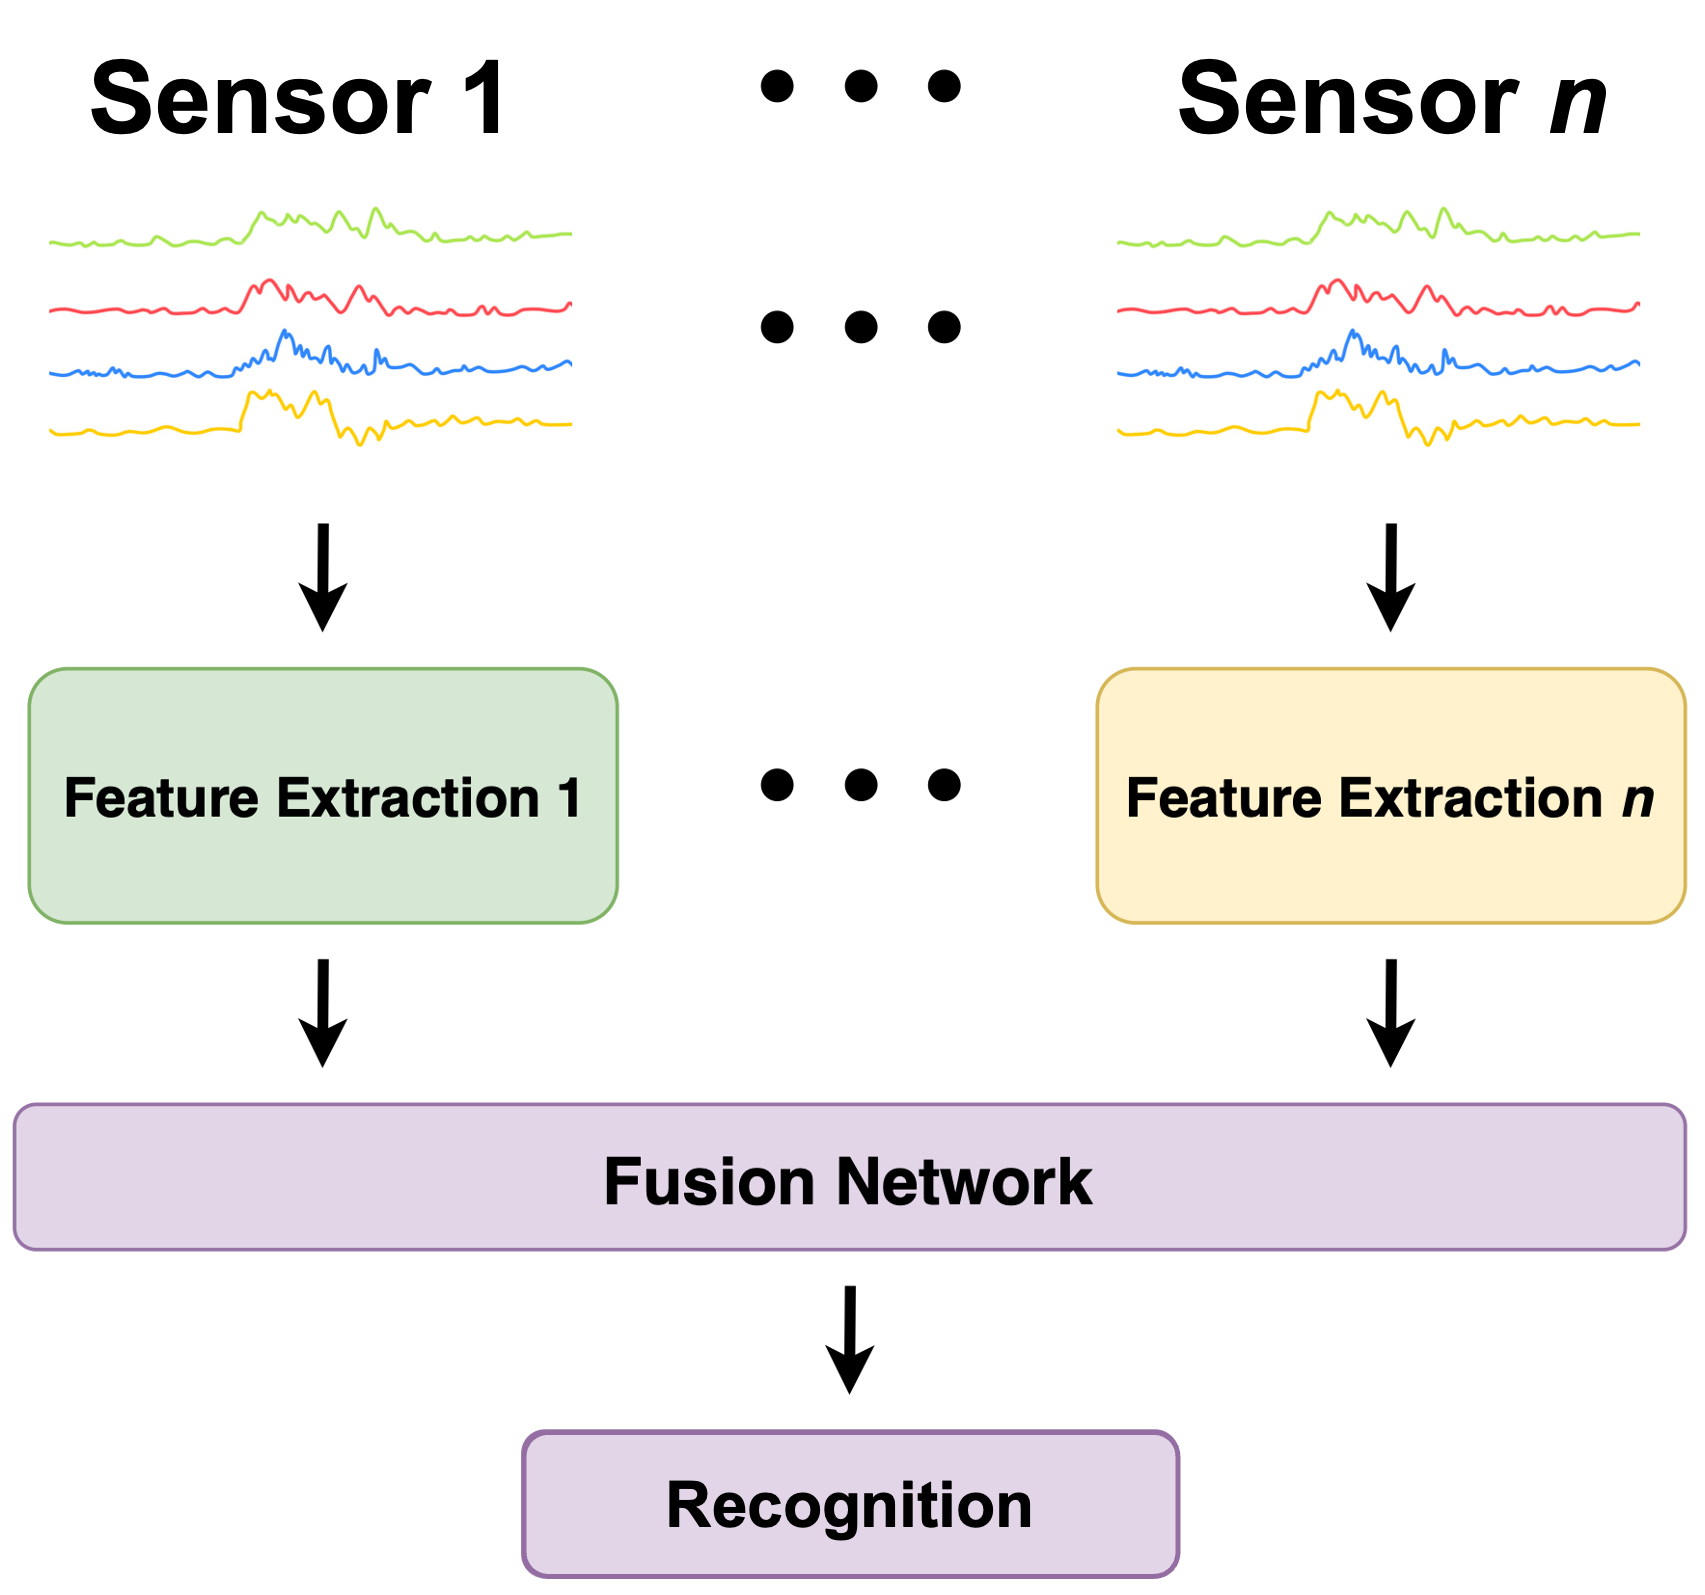
\includegraphics[width=0.4\columnwidth]{fig/sensor-and-fusion-networks.png}
    \caption{The model architecture in a nutshell: Using subnetworks for feature extraction of the different sensors (accelerometer, gyroscope, and \ac{gps}) and afterwards a fusion network to combine the features for final incident recognition~\cite{chen2021deep}.}
    \label{fig:sfn}
\end{figure}

The last big component of CycleSense is a \ac{rnn}.
\ac{rnn} architectures such as \ac{lstm}~\cite{hochreiter1997long} or \acp{gru}~\cite{chung2014empirical} are capable of holding information the network has seen before and using it to make predictions in the current state. 
In doing so, it is possible to identify patterns or relationships inside the timestamps of a bucket or between buckets. 
Similar to Yao et al.\ \cite{yao2017deepsense}, we also chose stacked \ac{gru} cells as they efficiently improve the model capacity~\cite{goodfellow2016deep}.

To determine the optimal set of parameters for training CycleSense, we have conducted a grid search on a variety of hyperparameters, some of which are shown in Figure~\ref{fig:hpo}.

In the following, we use \ac{gps}, accelerometer, and gyroscope data as model input if not indicated otherwise.  
Linear accelerometer data was only used in a few experiments as it is not available in our iOS and older Android data sets.
Our implementation of CycleSense is available on GitHub\footnote{https://github.com/simra-project/CycleSense}.

\begin{figure}[t]
	\centering
	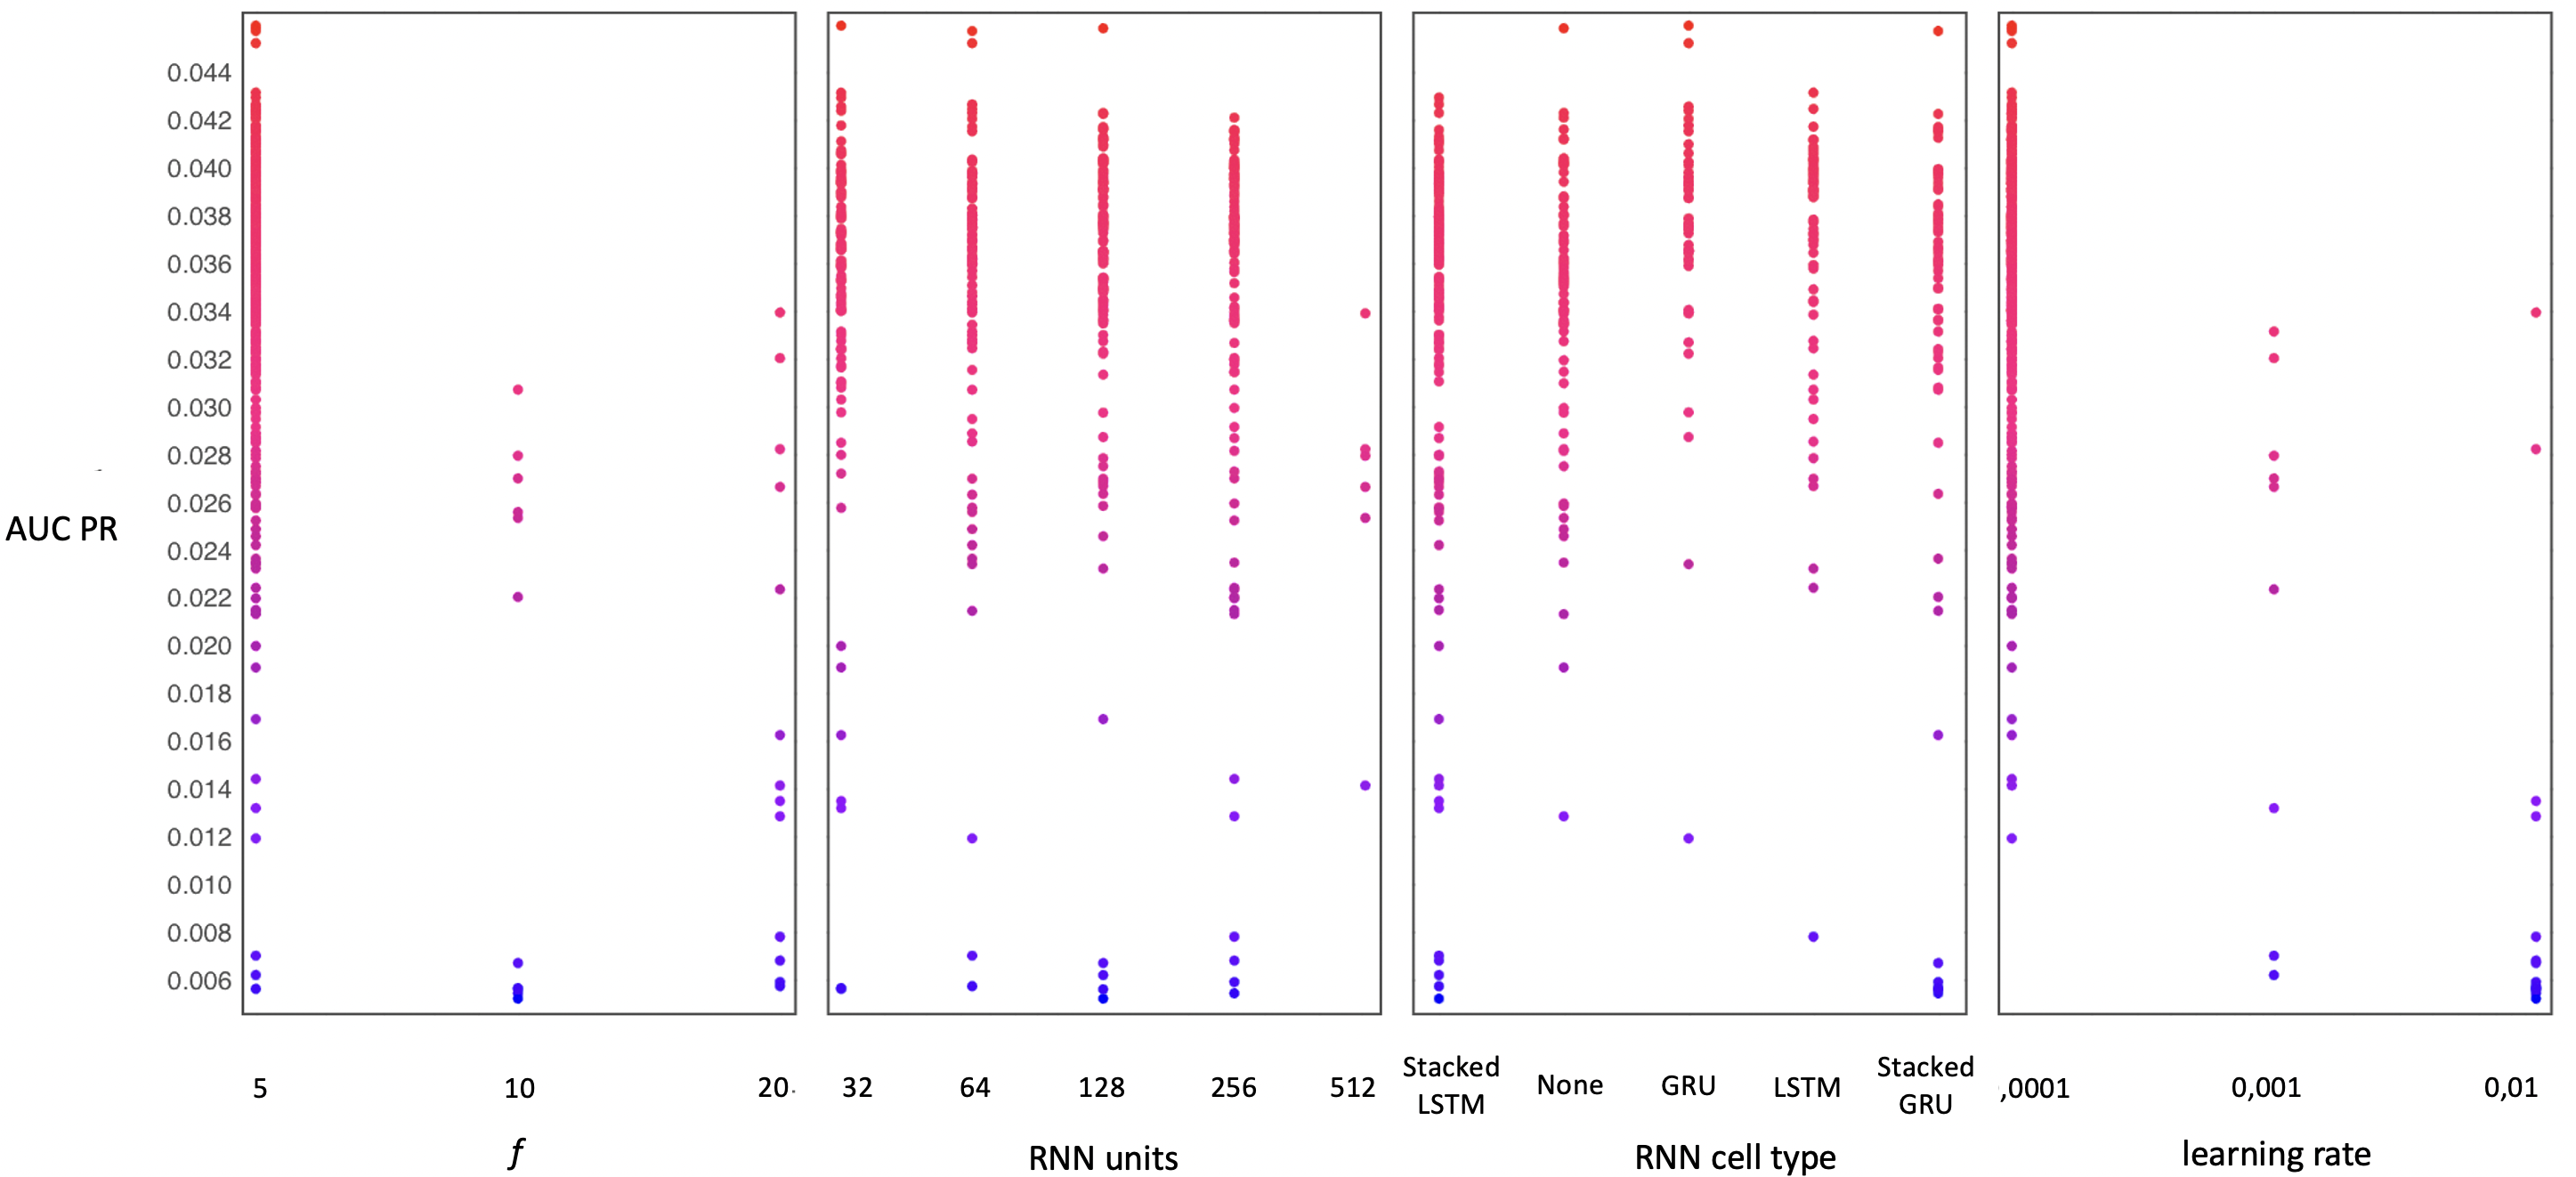
\includegraphics[width=\textwidth]{fig/hpo_results.png}
	\caption{Results of the hyperparameter optimization for the four variables $f$ (the window size), the number of \ac{rnn} units used, the \ac{rnn} cell type utilized, and the learning rate from left to right.}
	\label{fig:hpo}
\end{figure}

\subsection{Model Training}
\label{subsec:model_training}
For model training, the data set was split randomly into a training set (60\%), a validation set (20\%), and a test set (20\%).
Furthermore, the exact same splits are used for each model to improve comparability.
We trained the final model for 60 epochs on an NVIDIA K80 GPU.
We utilized a \ac{bce} loss function that was updated with Adam optimization, a \ac{sgd} method, a learning rate of 0.0001, and early stopping with a patience value of 10 epochs on the \ac{auc} \ac{roc} of the validation set.
It is important to note that we did not use the complete SimRa data set.
Instead, we used only a smaller subset of more recent rides recorded on Android devices since the heterogeneity of the data set across different versions and operating systems (see Section \ref{sec:discussion_cyclequality}) did not allow us to train a model properly on the full data set.
In addition, due to limited access to hardware, we focused predominantly on data originating from the Berlin region if not stated otherwise.

As previously described, one notable challenge we were facing was the extreme label imbalance present in the data.
This is due to the fact that incident buckets are far rarer than non-incident buckets.
To cope with that, we trained our model by using a weighted loss function with the class weights of the train data set as weights.
For example, the class weights were 1 and 170 for the rides that have recently been recorded on Android devices.

While the DeepSense model was trained in a standard fashion, we use stacking during the training of CycleSense.
Stacking (or stacked generalization) is an ensemble learning method that combines the predictions of several different models in order to contribute equally to a collective prediction.

However, we are also not interested in equal contributions of the network since that could overvalue models with a poor performance.
We therefore changed the CycleSense model to an integrated stacking model by adopting the idea of stacked generalization~\cite{wolpert1992stacked}, where the fusion network acts as the meta-learner.
Also, we deviate from a pure stacking model.
This is the case, as the meta-learner does not get any classification output of the subnetworks as input aside from the latent features in the last layer of the subnetworks.
Thereby, the weights of the submodel layers that have been pretrained individually are loaded and frozen, so they are not updated during the training of the whole CycleSense model.
This learning procedure further improved our results as shown in Section~\ref{sec:discussion_cyclesense}.

\section{Evaluation}
\label{sec:evaluation_cyclesense}
To evaluate CycleSense' training results, we have to put them into context. 
For this purpose, we compare them to the two detection methods currently used in the app as discussed in Section~\ref{sec:deep_learning_background}.
We give an overview of the changes we made to the baseline methods with the goal of a fair comparison in Section~\ref{subsec:baselines}.
We also describe the metrics that we use to compare our model to the baseline methods (Section~\ref{subsec:data_acquisition}) before presenting the results of our evaluation (Section~\ref{subsec:evaluation_results}).


\subsection{Baselines}
\label{subsec:baselines}
The first baseline is our original heuristic~\cite{karakaya2020simra} which is based on the underlying assumption that incidents will often result in sudden acceleration spikes, e.g., when braking or swerving to avoid obstacles.
We made some small changes to this heuristic to enable its compatibility with the \ac{auc} \ac{roc} metric, thus, increasing the comparability with our approach.

As a second baseline, we retrained the \ac{fcn} model from the alternative approach~\cite{sanchez2020detecting}.
We used the original preprocessing pipeline (which differs significantly from the here presented one) but used the full data set as introduced in Section~\ref{subsec:simra}.
We skipped the under-sampling step, disregarded the phone location and the bike type feature for the reasons mentioned in Section~\ref{subsec:preprocessing}, and used a non-overlapping sliding window approach with 10 second windows for better comparability.

The third baseline is DeepSense~\cite{yao2017deepsense}, which we implemented and trained as the authors describe in their work.
For the differences between DeepSense and CycleSense, see sections~\ref{subsec:model_architecture} and~\ref{sec:related_work_cyclesense}.

Based on these changes for improved comparability, we retrained the original model.
We use both baselines for comparison as they are, to our knowledge, the only approaches for (semi-)automatically detecting incidents based on sensory time series data.
Furthermore, they have been developed on the SimRa data set, which enables a fair comparison.

\subsection{Metrics}
\label{subsec:metrics}
Due to the massive label imbalance already mentioned earlier, common metrics such as accuracy, F1-score, and precision are difficult to interpret.
Moreover, in our scenario it is more important to find the true incidents than to classify non-incidents correctly, as False Positives can be more easily corrected by the user of the SimRa app.
For both reasons, a high number of False Positives is more acceptable than a low number of True Positives, which further limits the usefulness of such metrics like precision, F1-score, or \ac{mcc}.
Therefore, we focus on the \ac{auc} of the \ac{roc} metric, which is insensitive to changes in class distribution~\cite{fawcett2006introduction} while also reporting the respective confusion matrices.

\subsection{Evaluation Results}
\label{subsec:evaluation_results}
In a first step, we compare CycleSense to the two baselines and common model architectures used in the context of \ac{dl} for \ac{tsc}~\cite{ismail2019deep}.
All of these were trained on the Android data set consisting of more recent rides which provides the best results for all approaches.
Figure~\ref{fig:roc-auc-results} and Table~\ref{tab:roc-auc-results} show the differences in performance.

The \ac{fcn} and CycleSense clearly outperform the modified heuristic (0.621 \ac{auc} \ac{roc}).
However, there is still a big performance gap between our model and the \ac{fcn} model.
While the \ac{fcn} model scores 0.847 \ac{auc} \ac{roc}, CycleSense achieves an \ac{auc} \ac{roc} score of 0.906, i.e., there is a chance of $\approx$ 90.6\% that the model can distinguish correctly between a randomly chosen incident and non-incident bucket.
Furthermore, our model performs better than other model architectures that are common for \ac{dl} in \ac{tsc}~\cite{ismail2019deep}: Auto Encoder, \ac{gaf}, \ac{esn}, and the \ac{cnn}-\ac{lstm} model.
With regard to the increasing model complexity, we clearly see diminishing returns.
We can see this in the example of the rather simple \ac{cnn}-\ac{lstm} model which exhibits a relatively close performance to the much more complex CycleSense model with stacking.
The \ac{cnn}-\ac{lstm} model has $\approx$ 90,000 parameters, while the CycleSense model has $\approx$ 1,100,000 parameters.
As a consequence, the time to evaluate the test set of the newer Android data consisting of 795 rides took 4 seconds with the \ac{cnn}-\ac{lstm} model and 56 seconds using CycleSense on the NVIDIA GPU.

\begin{figure}[t]
	\centering
	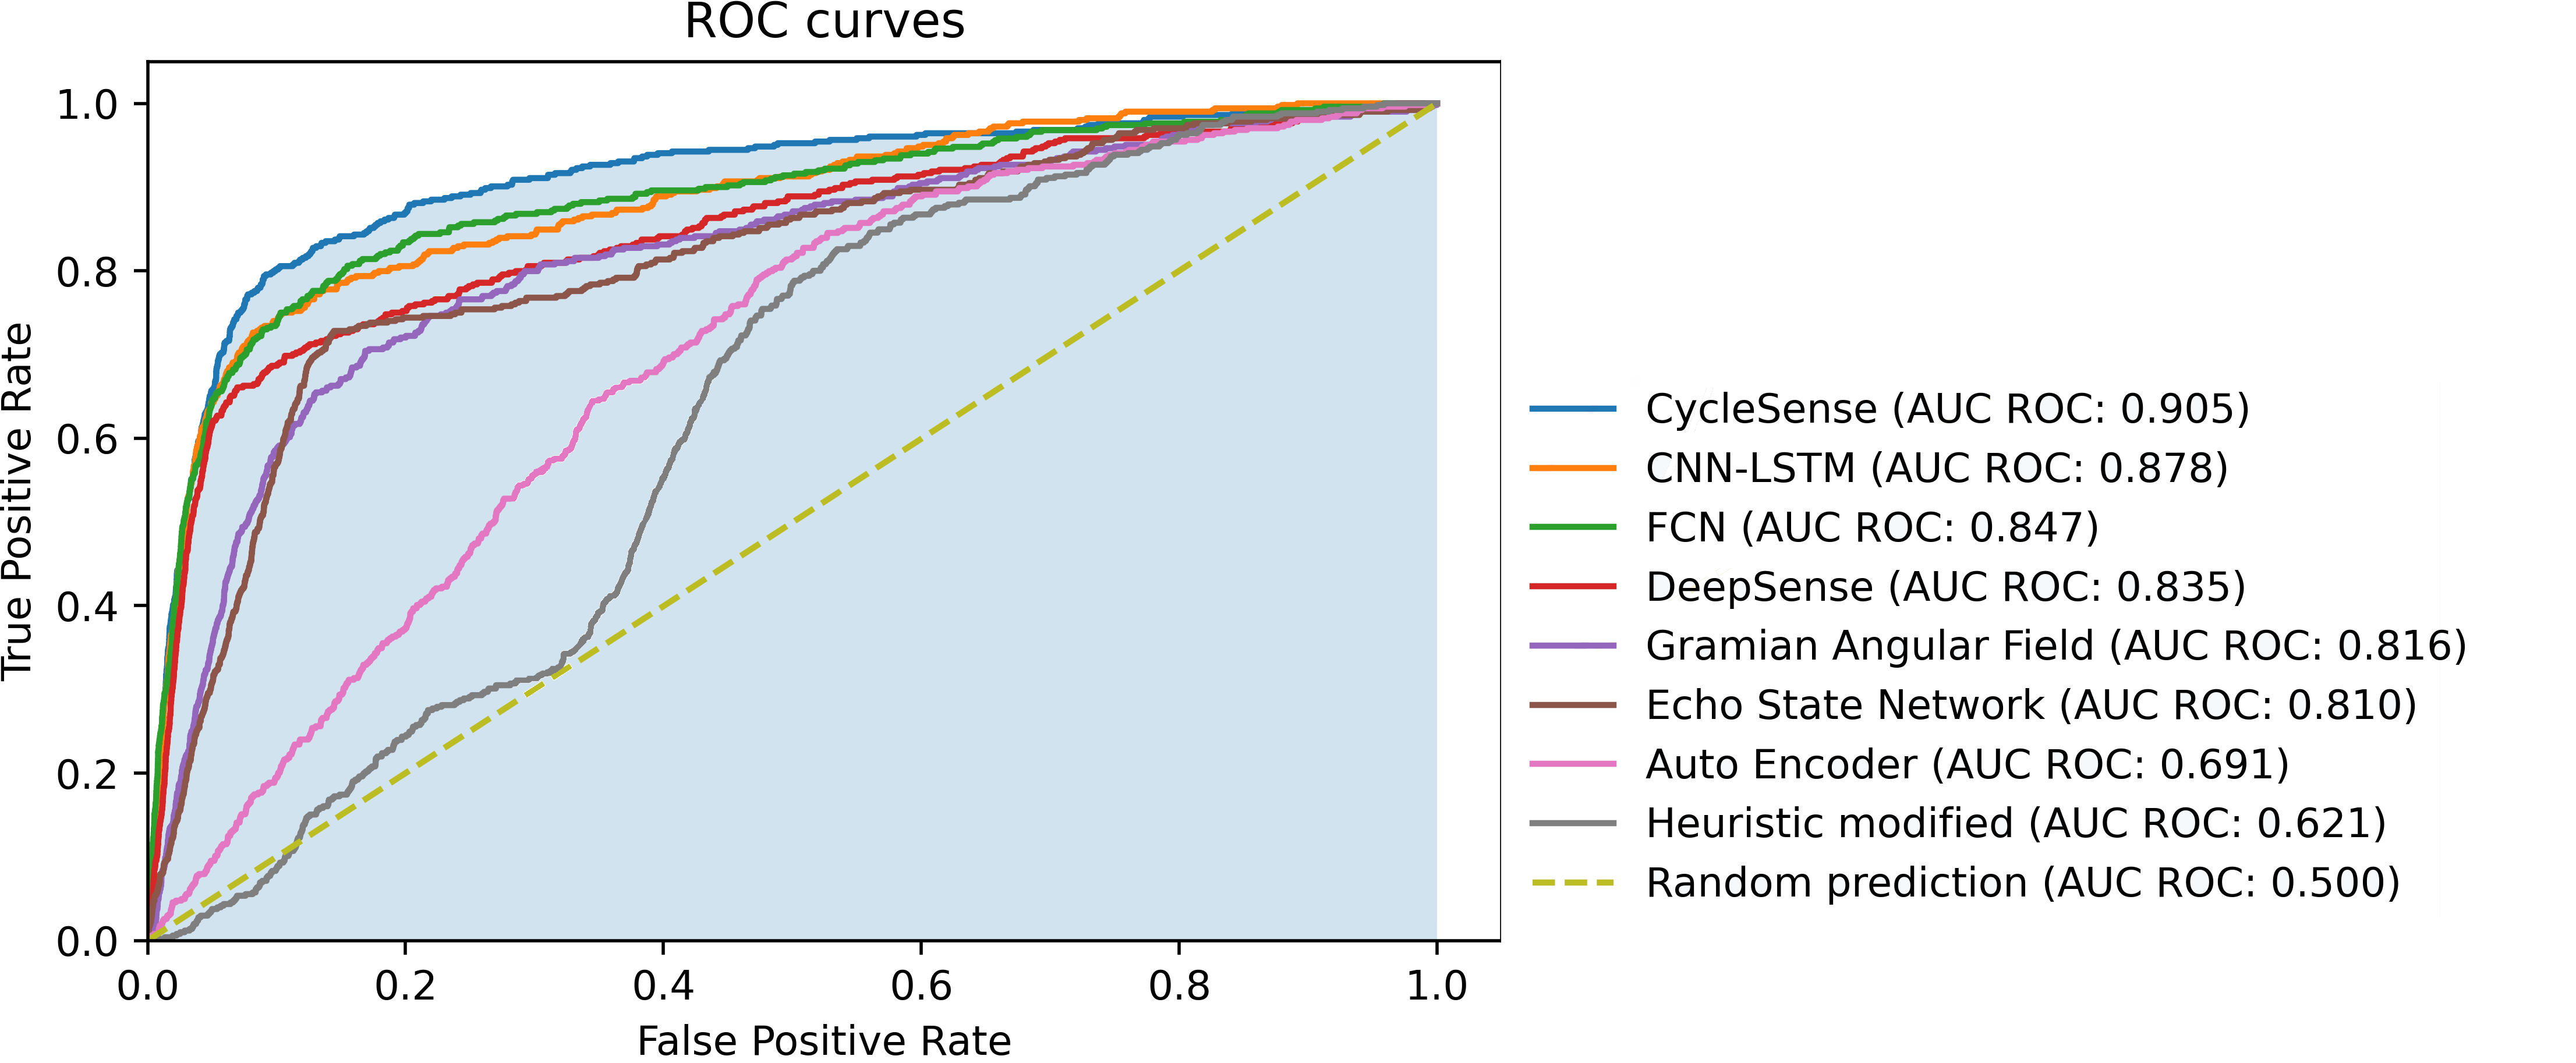
\includegraphics[width=0.8\textwidth]{fig/roc_auc_results_legend.png}
	\caption{Comparison of the baselines and common model architectures used in the context of \ac{dl} for \ac{tsc}~\cite{ismail2019deep} with the CycleSense model. Note that all of these models have been trained and evaluated on rides contained in the SimRa data set that have been recorded with more recent versions of the SimRa Android app.}
	\label{fig:roc-auc-results}
\end{figure}

\begin{table}
	\centering
	\resizebox{\columnwidth}{!}{%
	\begin{tabular}{cccccccccc}
		\hline
		\centering
		& \textbf{TN} & \textbf{FP} & \textbf{FN} & \textbf{TP} & \textbf{\ac{auc} \ac{roc}} & \textbf{Precision} & \textbf{Recall} & \textbf{F1-Score} & \textbf{MCC} \\
		\hline\hline
		\textbf{CycleSense} & 107934 & 10893 & 104 & 400 & \cellcolor{yellow}0.906 & \cellcolor{yellow}0.035 & 0.794 & \cellcolor{yellow}0.068 & \cellcolor{yellow}0.156 \\
		\hline
		\textbf{CNN-LSTM} & 106427 & 12400 & 127 & 377 & 0.878 & 0.030 & 0.748 & 0.057 & 0.135 \\
		\hline
		\textbf{FCN} & 100932 & 18500 & 98 & 402 & 0.847 & 0.021 & \cellcolor{yellow}0.804 & 0.041 & 0.115 \\
		\hline
		\textbf{DeepSense} & 106192 & 12635 & 153 & 351 & 0.835 & 0.027 & 0.696 & 0.052 &  0.123 \\
		\hline
		\textbf{GAF} & 98782 & 20045 & 150 & 354 & 0.816 & 0.017 & 0.702 & 0.034 & 0.092 \\
		\hline
		\textbf{ESN} & 101670 & 17157 & 138 & 366 & 0.810 & 0.021 & 0.726 & 0.041 & 0.107 \\
		\hline
		\textbf{Auto Encoder} & 58416 & 60411 & 88 & 416 & 0.691 & 0.007 & 0.825 & 0.014 & 0.041 \\
		\hline
	\end{tabular}%
}
\caption{Comparison of the baselines and common model architectures used in the context of \ac{dl} for \ac{tsc}~\cite{ismail2019deep} with the CycleSense model. See the discussion in Section~\ref{subsec:metrics} about the usefulness of various metrics. Note also that all of these models have been trained and evaluated on rides contained in the SimRa data set that have been recorded with more recent versions of the SimRa Android app. For all models the threshold which optimizes Youden's index\cite{youden1950index} were chosen.}
\label{tab:roc-auc-results}
\end{table}

In another experiment, we include the linear accelerometer sensor values in addition to the accelerometer, gyroscope and \ac{gps} data we used so far.
The result for CycleSense is again an \ac{auc} \ac{roc} of 0.906, although the model requires more memory, training and processing time.
Therefore, we leave out the linear accelerometer feature.

So far, we have predominantly focused on newer rides recorded on the Android version of the SimRa app.
As shown in Figure~\ref{fig:traindonone}, the model performs far worse on the other splits of the data set.
Therefore, it was necessary to train an individual model for each part of the data set. 
This yields far better results (Figure~\ref{fig:individually}).

\begin{figure}[t]
	\centering
	\begin{subfigure}[b]{0.475\textwidth}
		\centering
		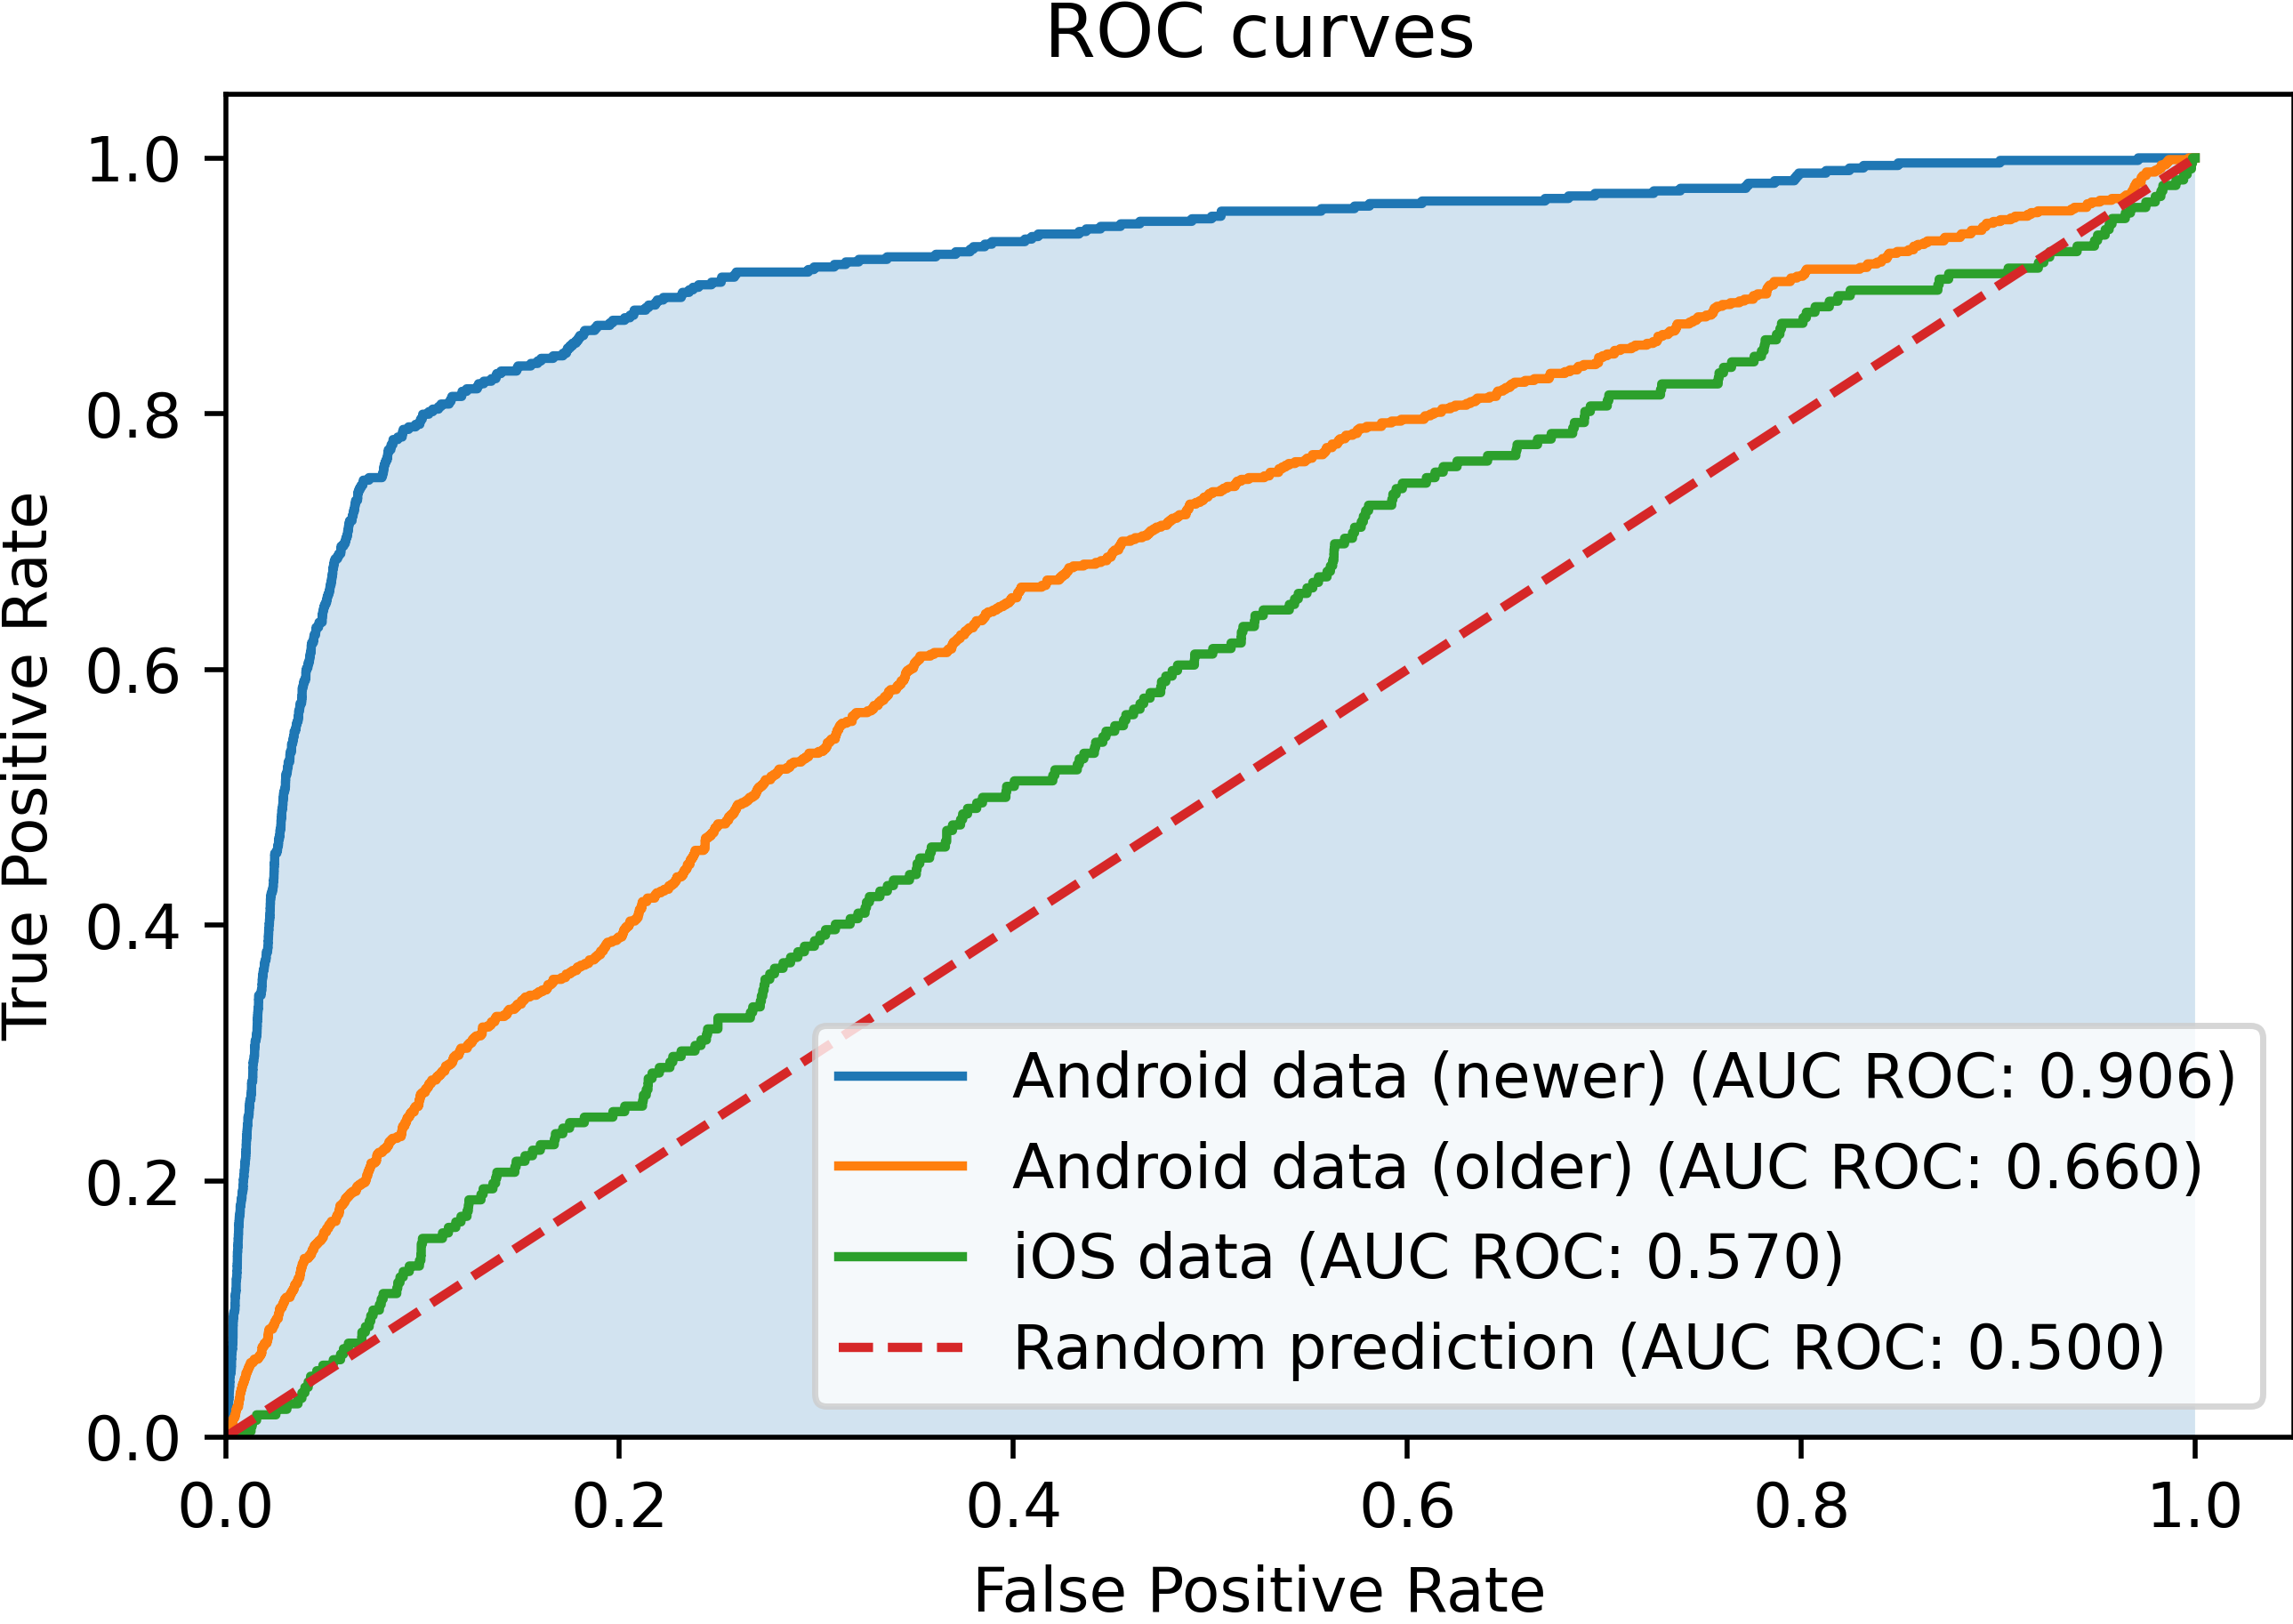
\includegraphics[width=\textwidth]{fig/rocauctrainedon73.png}
		\caption{\small CycleSense trained only on the newer Android rides and evaluated on all parts of the data set.}
		\label{fig:traindonone}
	\end{subfigure}
	\hfill
	\begin{subfigure}[b]{0.475\textwidth}
		\centering
		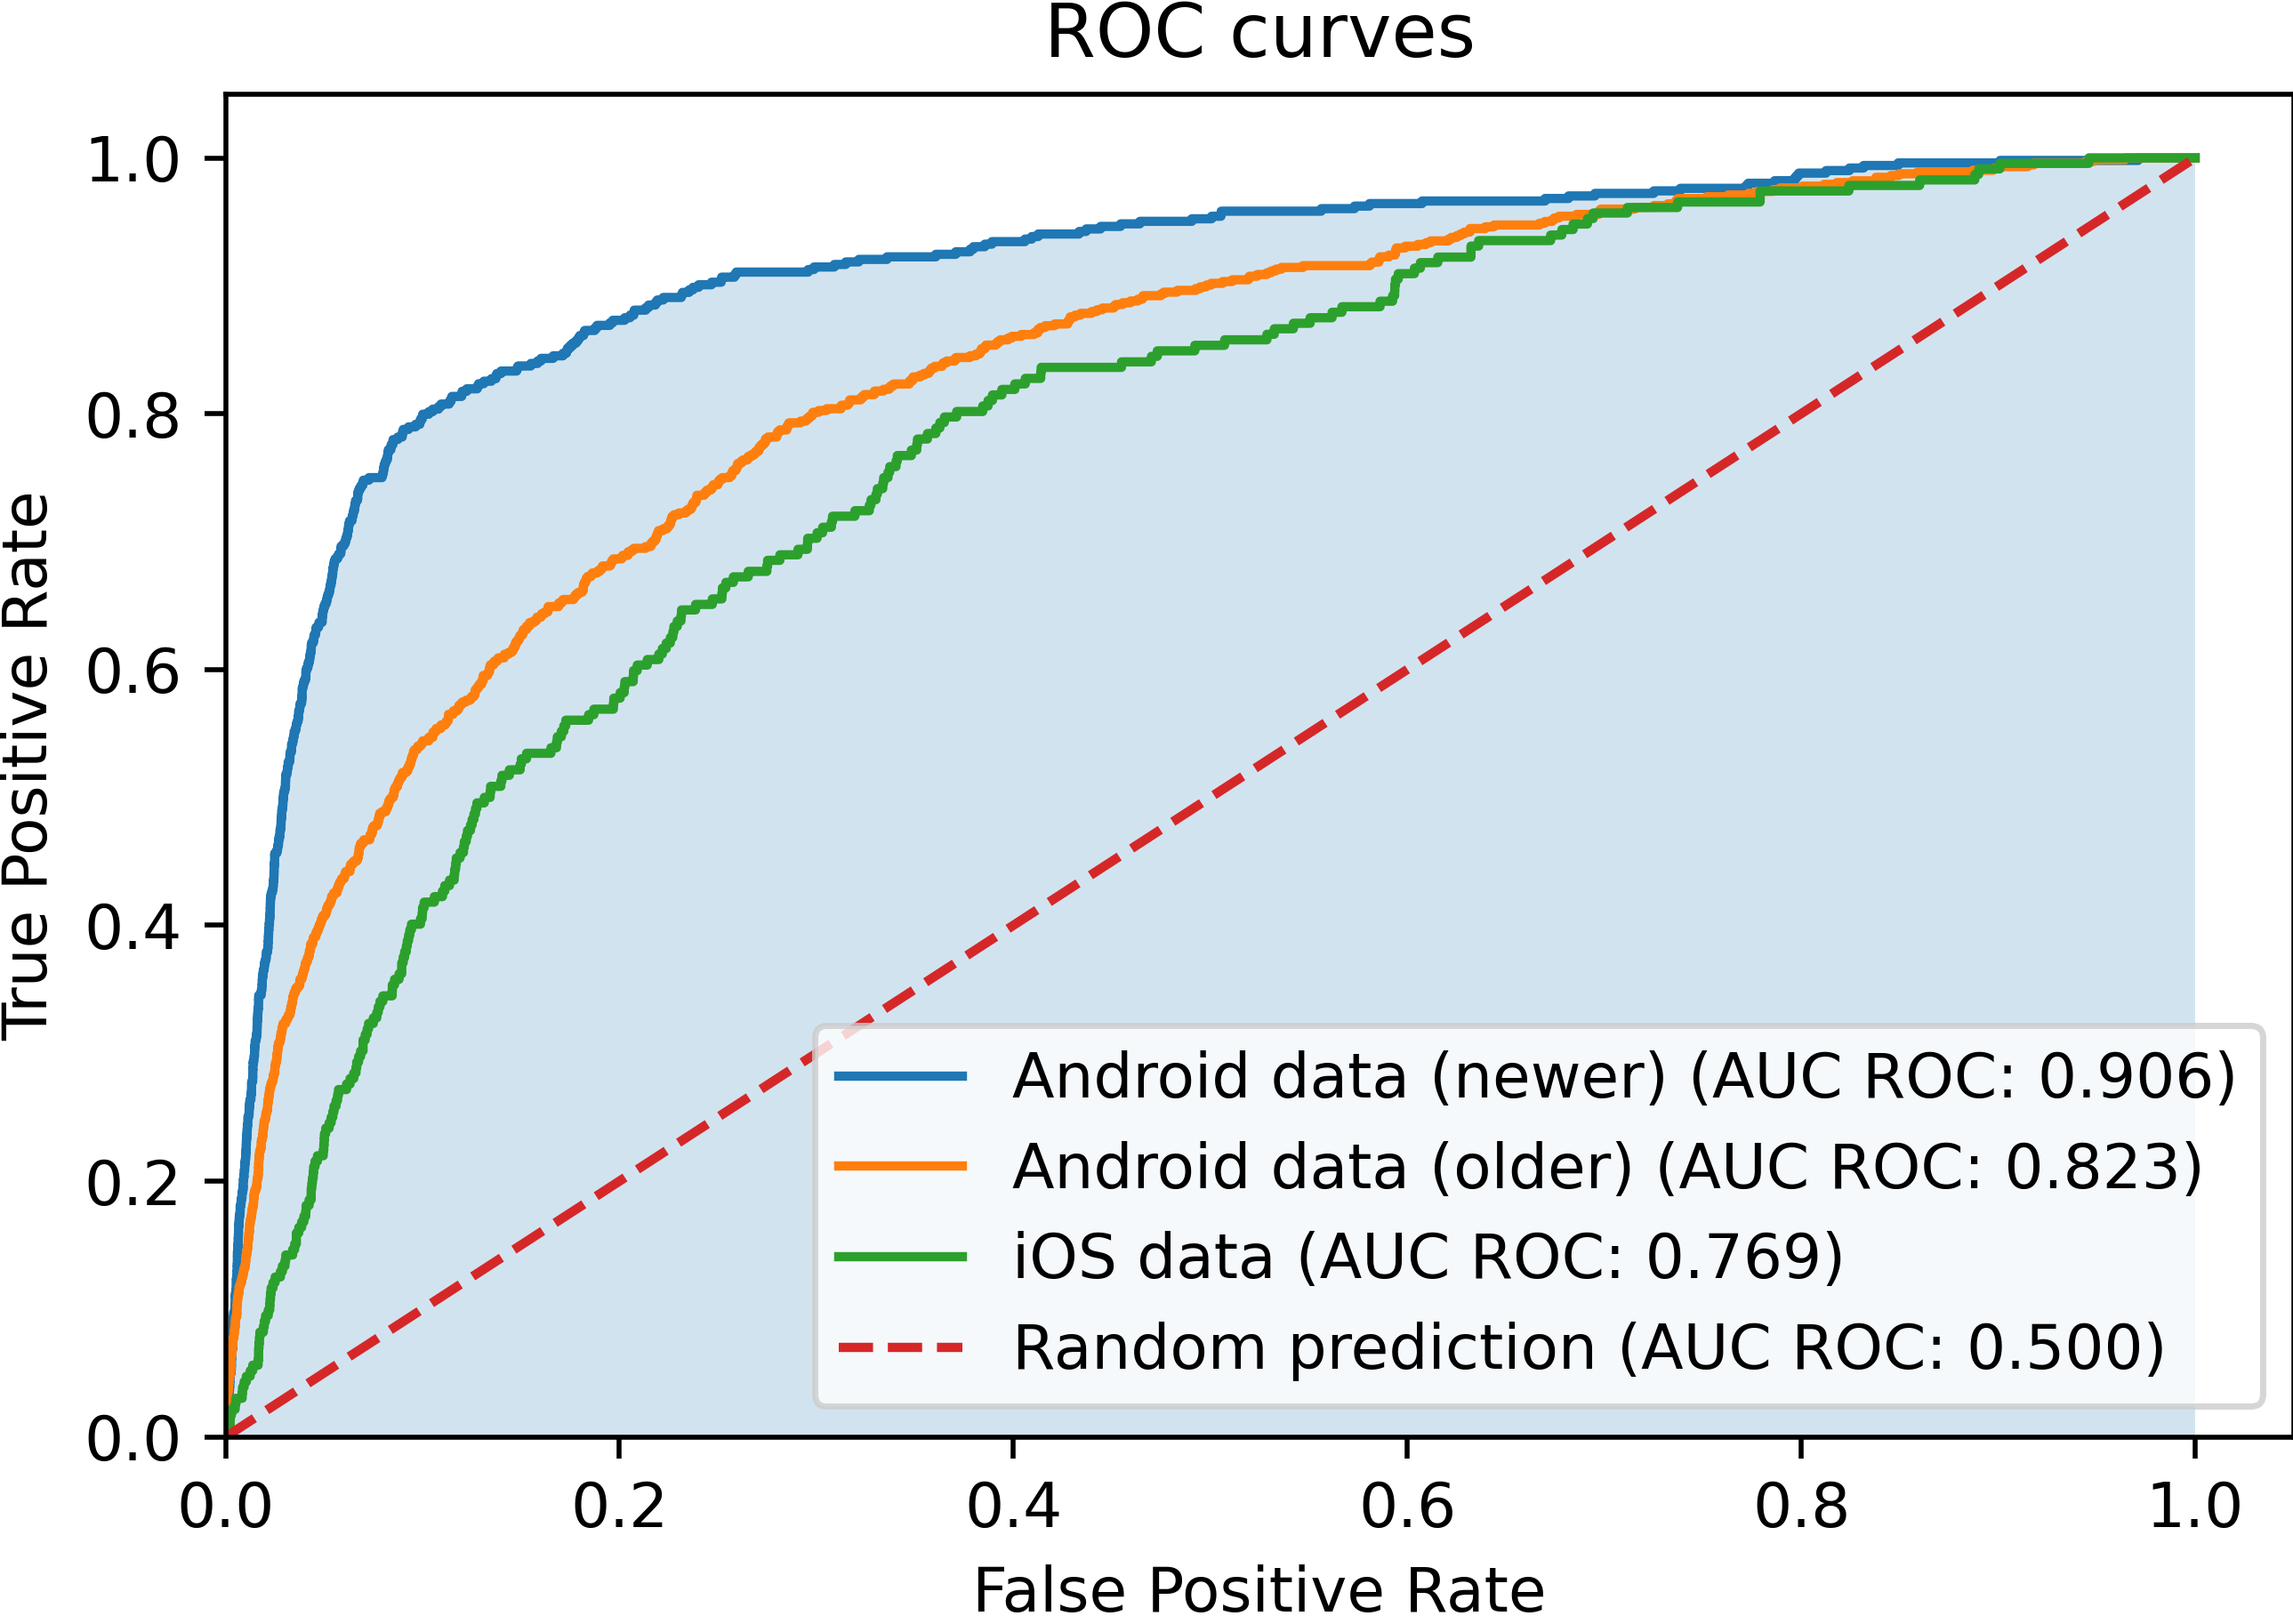
\includegraphics[width=\textwidth]{fig/rocauctrainedindividually.png}
		\caption{\small CycleSense trained and evaluated individually on all parts of the data set. \newline}
		\label{fig:individually}
	\end{subfigure}
	\caption{Comparison of CycleSense trained only on the newer Android rides or individual CycleSense models trained for each part of the data set. Note that only the newer Android data set was manually cleaned.}
	\label{fig:comp-trainedonone-individually}
\end{figure}

As the Berlin region has by far recorded the most rides, we have so far used only those for tuning, training, and evaluating our model.
The SimRa app, however, is deployed in many more regions, so our model is clearly required to perform there, too.
For this reason, we have evaluated the Berlin CycleSense model on the newer Android rides coming from Hanover and Nuremberg.

The outcome of this experiment is visualized in Figure~\ref{fig:different-city-trained-on-berlin}.
It clearly shows, that CycleSense does not perform as good as in Berlin.
Since most regions lack training data, it would not be a feasible solution to train models individually per region in the current stage of the SimRa project.
Instead, we retrain CycleSense on a data set that includes all the rides recorded on the newer versions of the Android app within the Berlin, Nuremberg, and Hanover regions.
The results from Figure~\ref{fig:different-city-trained-individually} show that this clearly improves the performance in these additional regions.
At the same time, the performance on the Berlin data set has declined only slightly (0.029 \ac{auc} \ac{roc}) by comparison.
Nevertheless, the \ac{auc} \ac{roc} for Berlin is still the highest and clearly above Nuremberg, which is well ahead of Hanover.

\begin{figure}[t]
	\centering
	\begin{subfigure}[b]{0.475\textwidth}
		\centering
		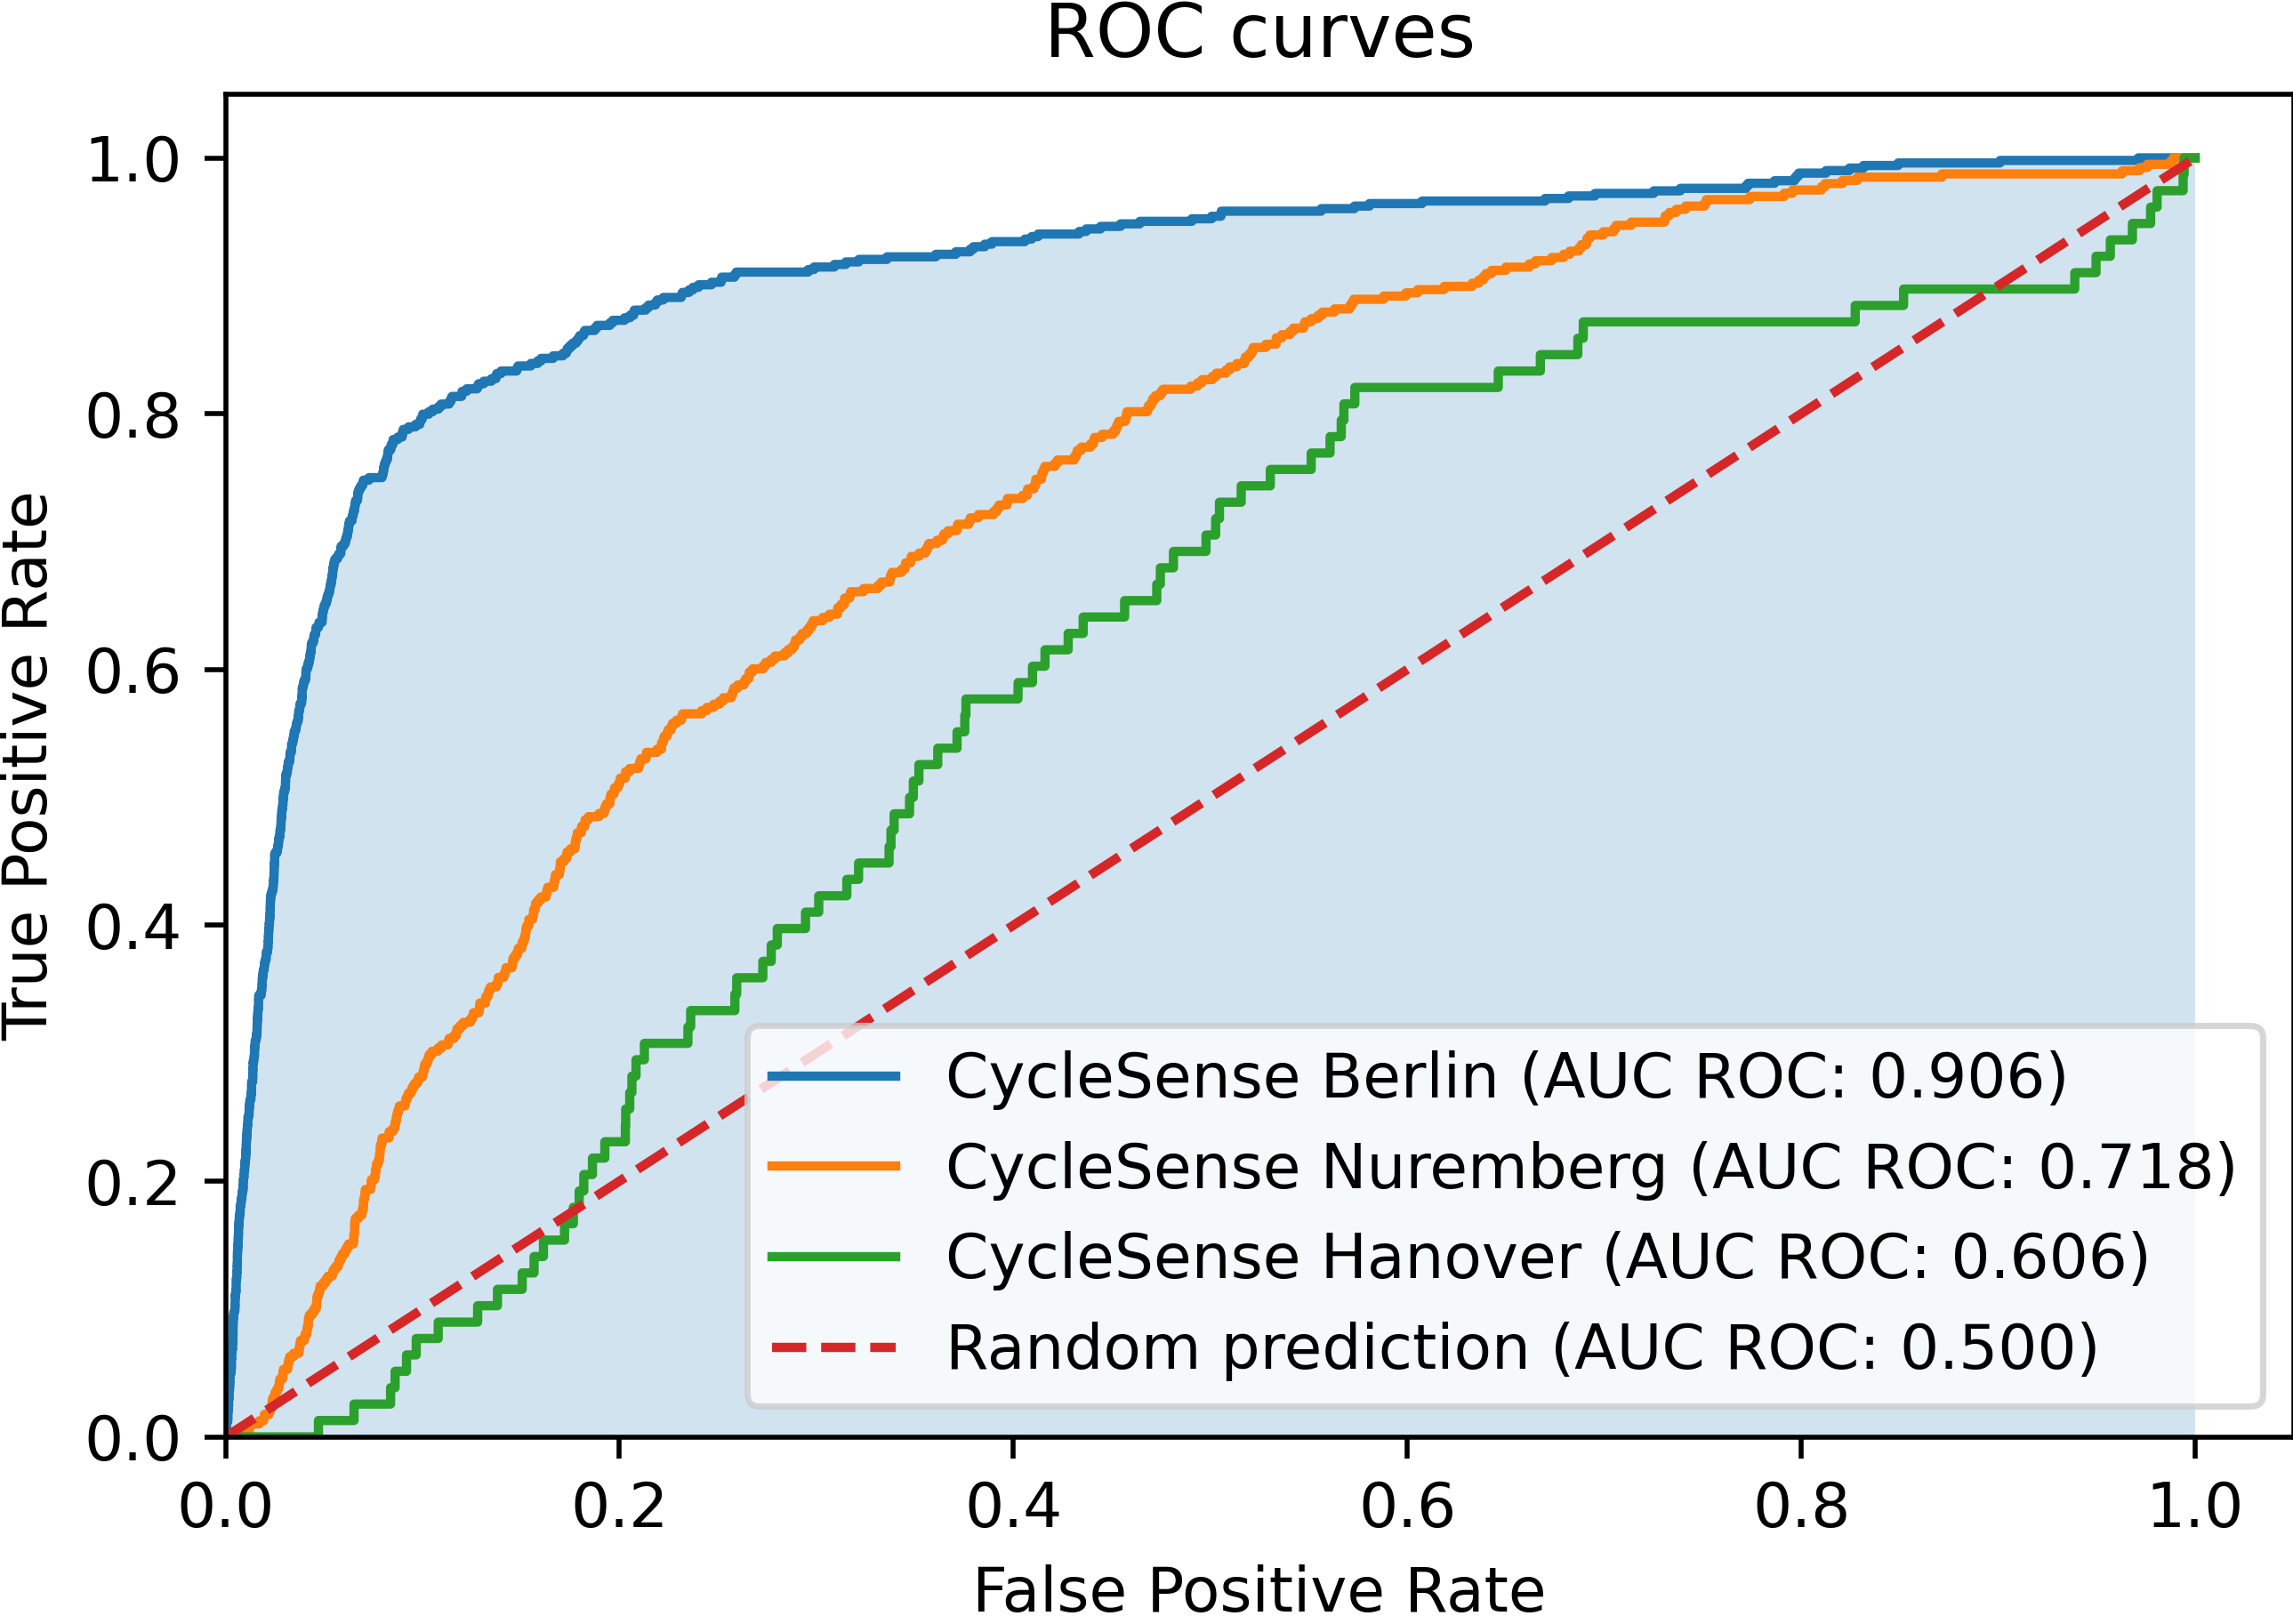
\includegraphics[width=\textwidth]{fig/city_comp_before.png}
		\caption{\small Performance of CycleSense trained on the new Android data set of rides recorded in Berlin. \newline}
		\label{fig:different-city-trained-on-berlin}
	\end{subfigure}
	\hfill
	\begin{subfigure}[b]{0.475\textwidth}
		\centering
		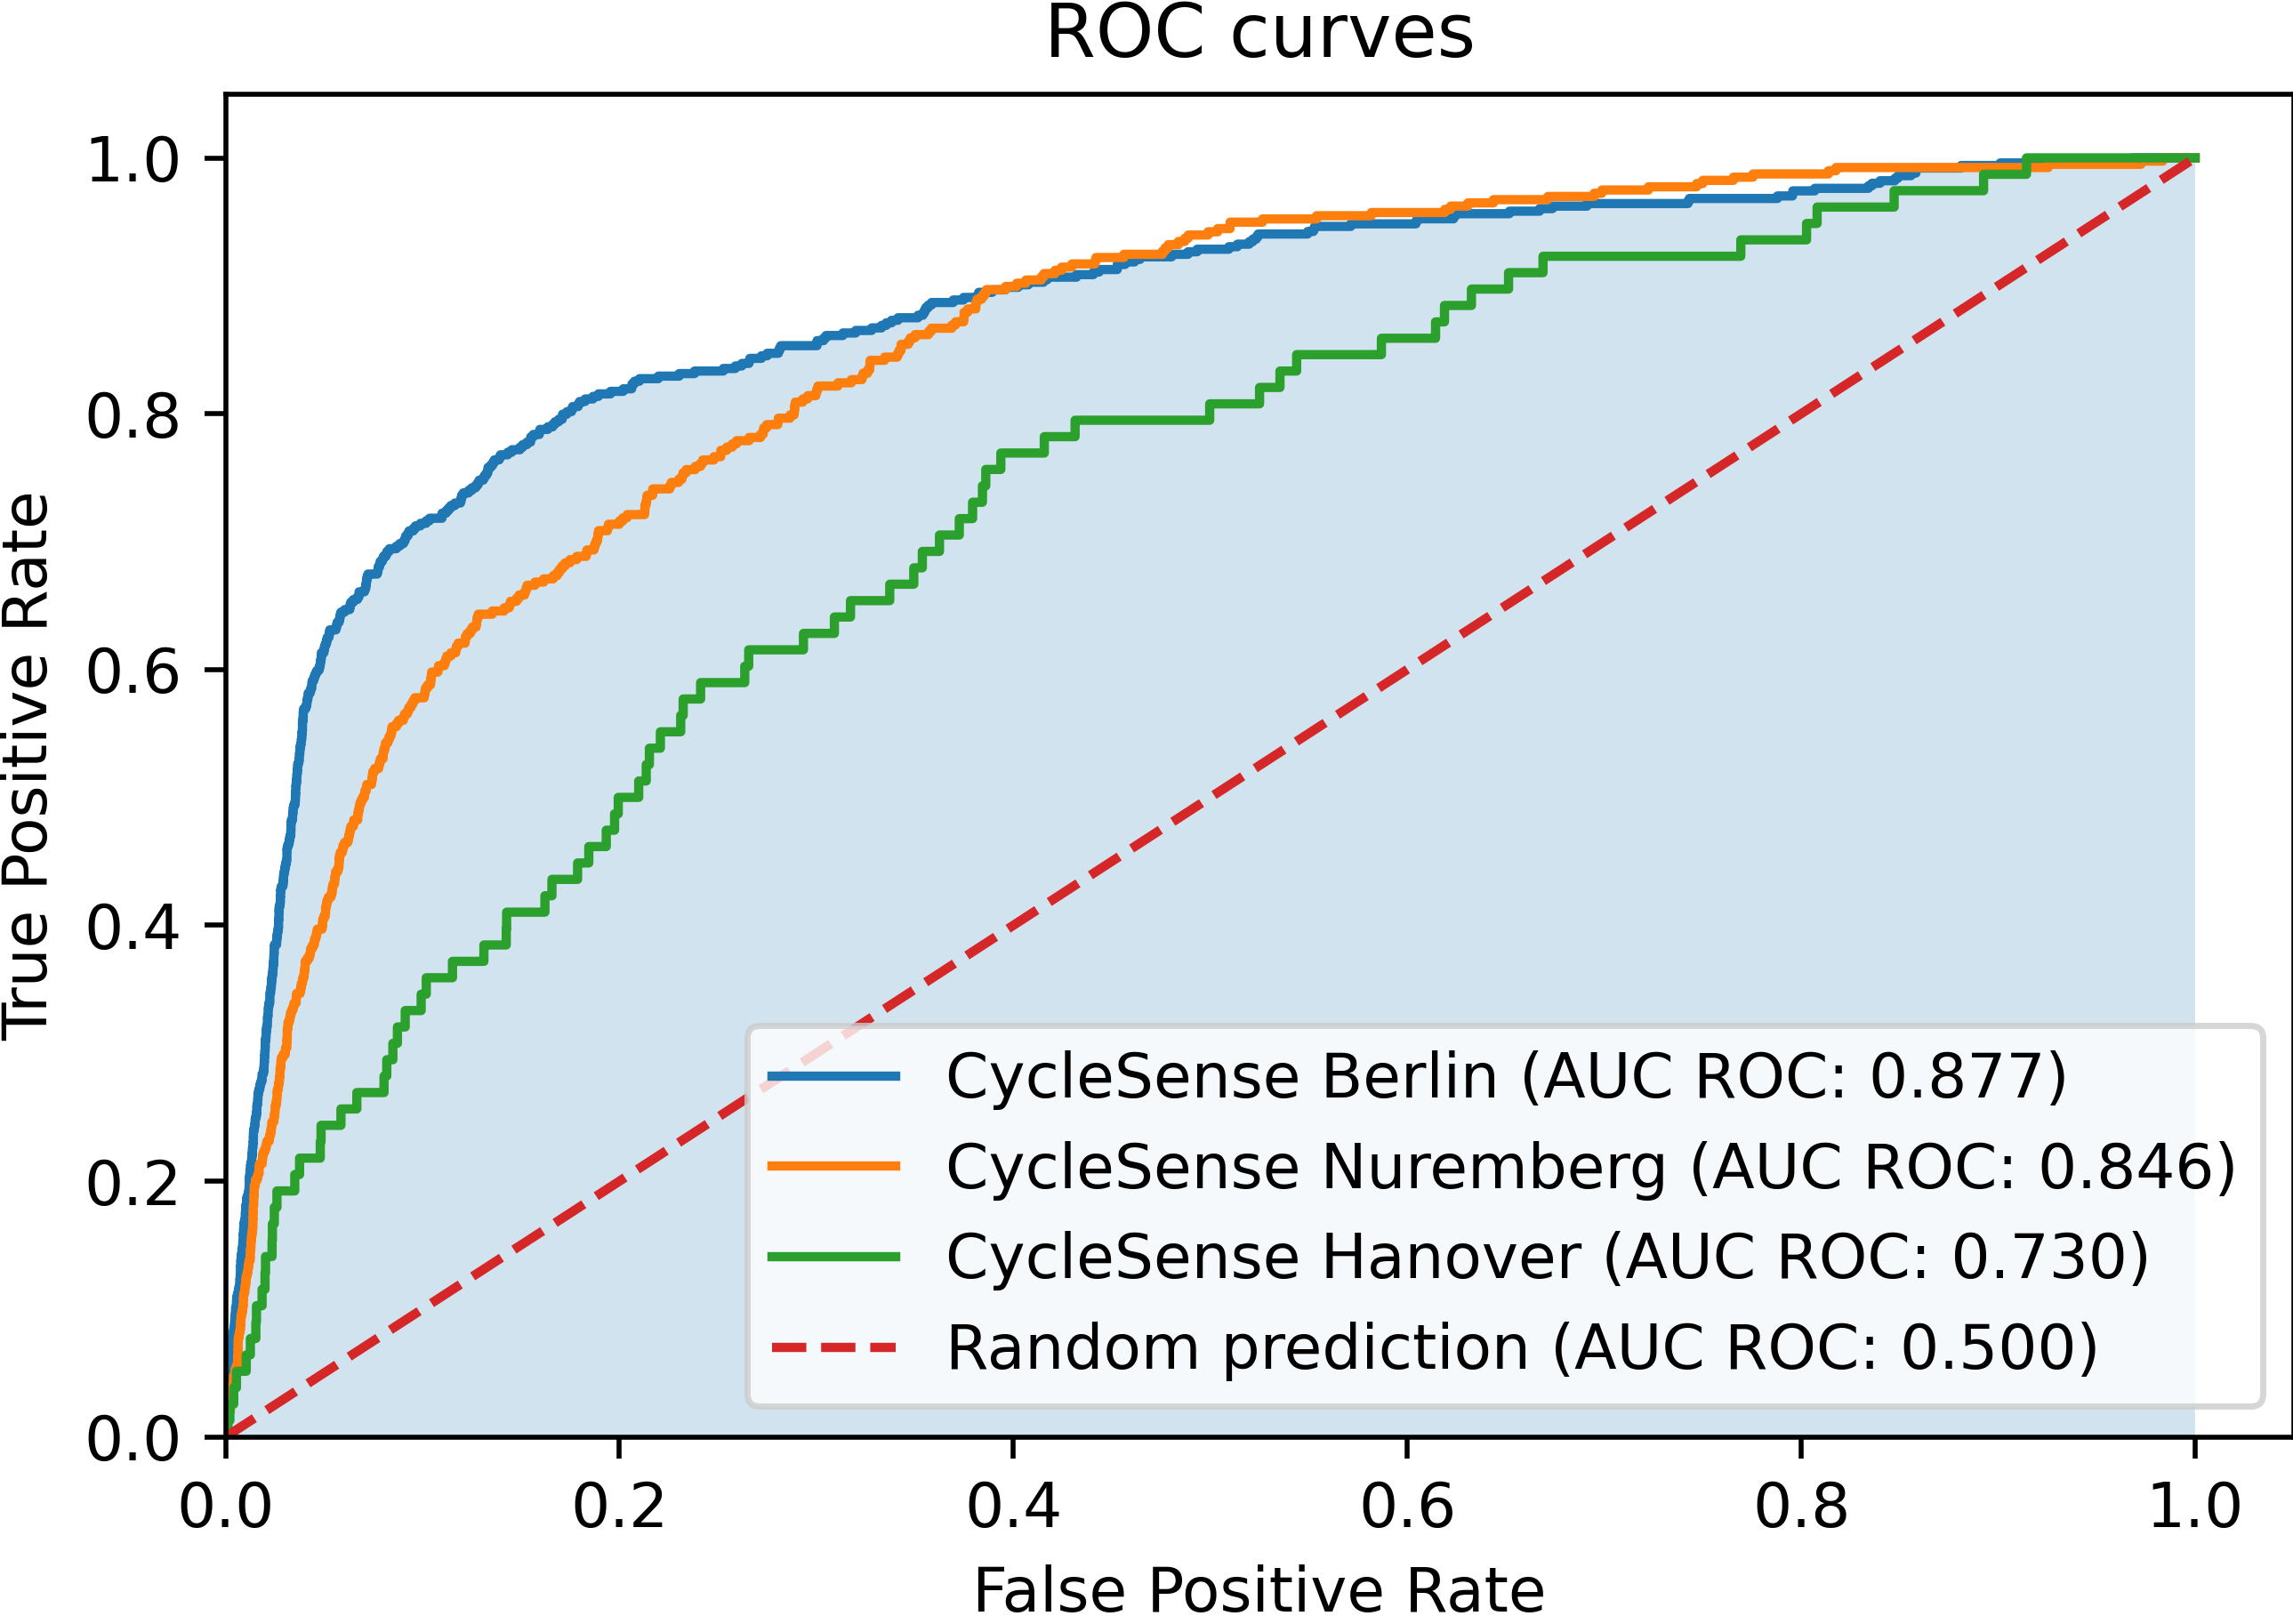
\includegraphics[width=\textwidth]{fig/city_comp_after.png}
		\caption{\small Performance of CycleSense trained on the new Android data set of rides recorded in Berlin, Nuremberg, and Hanover.}
		\label{fig:different-city-trained-individually}
	\end{subfigure}
	\caption{Comparison of the performance of CycleSense trained on Berlin and trained on the other regions combined.}
\end{figure}

\section{Discussion}
\label{sec:discussion_cyclesense}
Our results demonstrate that the proposed CycleSense model outperforms every other model that we have compared to.
While improving the model's architecture and other components, we identified a number of challenges inherent to the problem setting that we discuss in the following.
Note that we also discuss some limitations in \cref{cha:discussion_and_outlook}, that may also apply to this approach.


\subsection{Impact of Preprocessing \& Training Steps}
\label{subsec:impact_of_preprocessing_and_training_steps}
In a first step, we want to highlight the importance of our preprocessing and training methods for the success of our model.
Therefore, Figure~\ref{fig:impact} illustrates the performance of CycleSense when one of the preprocessing or training methods is skipped, resulting in a significant drop in performance in each of the four examples.

\begin{figure}[t]
	\centering
	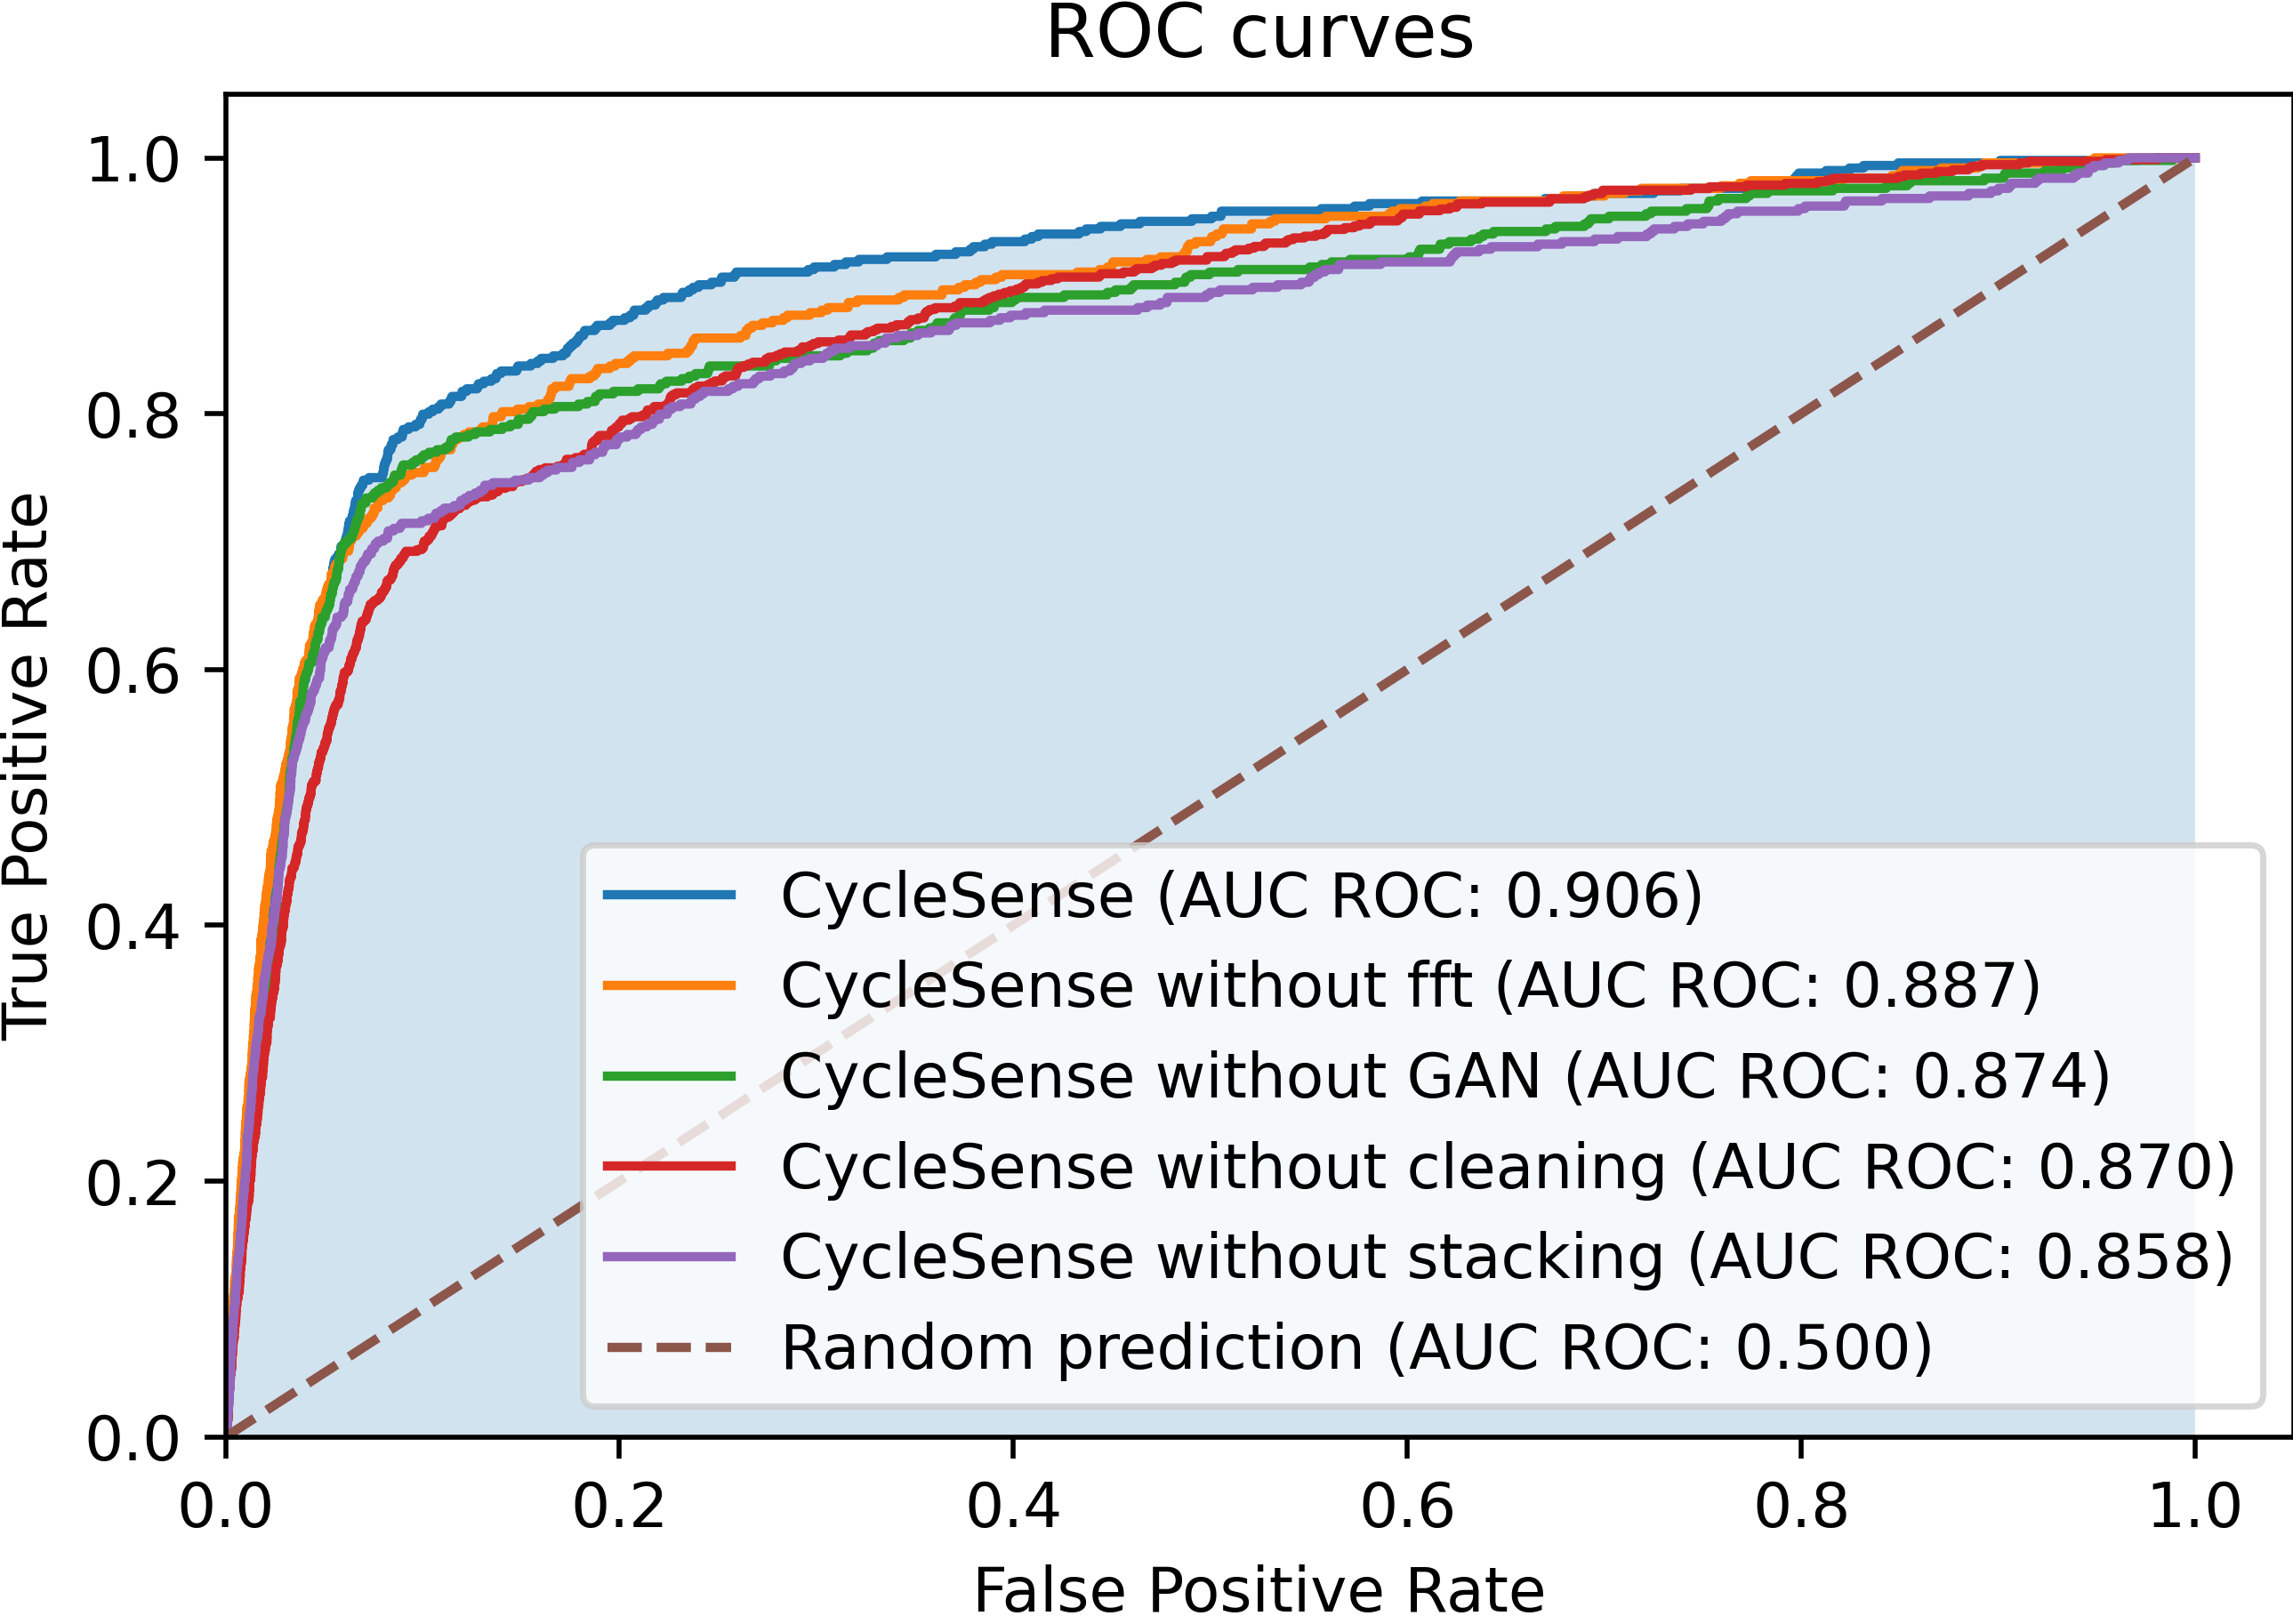
\includegraphics[width=0.5\textwidth]{fig/impact.png}
	\caption{Impact of different preprocessing and training steps on the performance of CycleSense.}
	\label{fig:impact}
\end{figure}

\subsection{Technical Limitations of the SimRa Data Set}
\label{subsec:technical_limitations_of_the_simra_data_set}
Recording rates of sensor readings deviate among devices and operating systems and impair model predictions~\cite{stisen2015smart}, this may also affect the performance of CycleSense:
As illustrated in Figure~\ref{fig:emp-measurements}, the recording rates differ significantly in older and newer Android rides as well as in iOS rides.
While the iOS rides' median ($\approx$ 300 ms) is similar to the one of newer Android rides, the \ac{iqr} is much greater and spans approximately 150 ms.
This circumstance could indicate that the relatively weak model performance on this data set can partly be explained by that factor. 
Furthermore, the gyroscope data is recorded with a higher frequency in newer Android rides than in older Android or iOS rides.
This factor could also contribute to the different model evaluation results. 
The achieved \ac{auc} \ac{roc} for uncleaned newer Android data was 0.870, while it was 0.823 for the older Android data.

\begin{figure}[t]
	\centering
	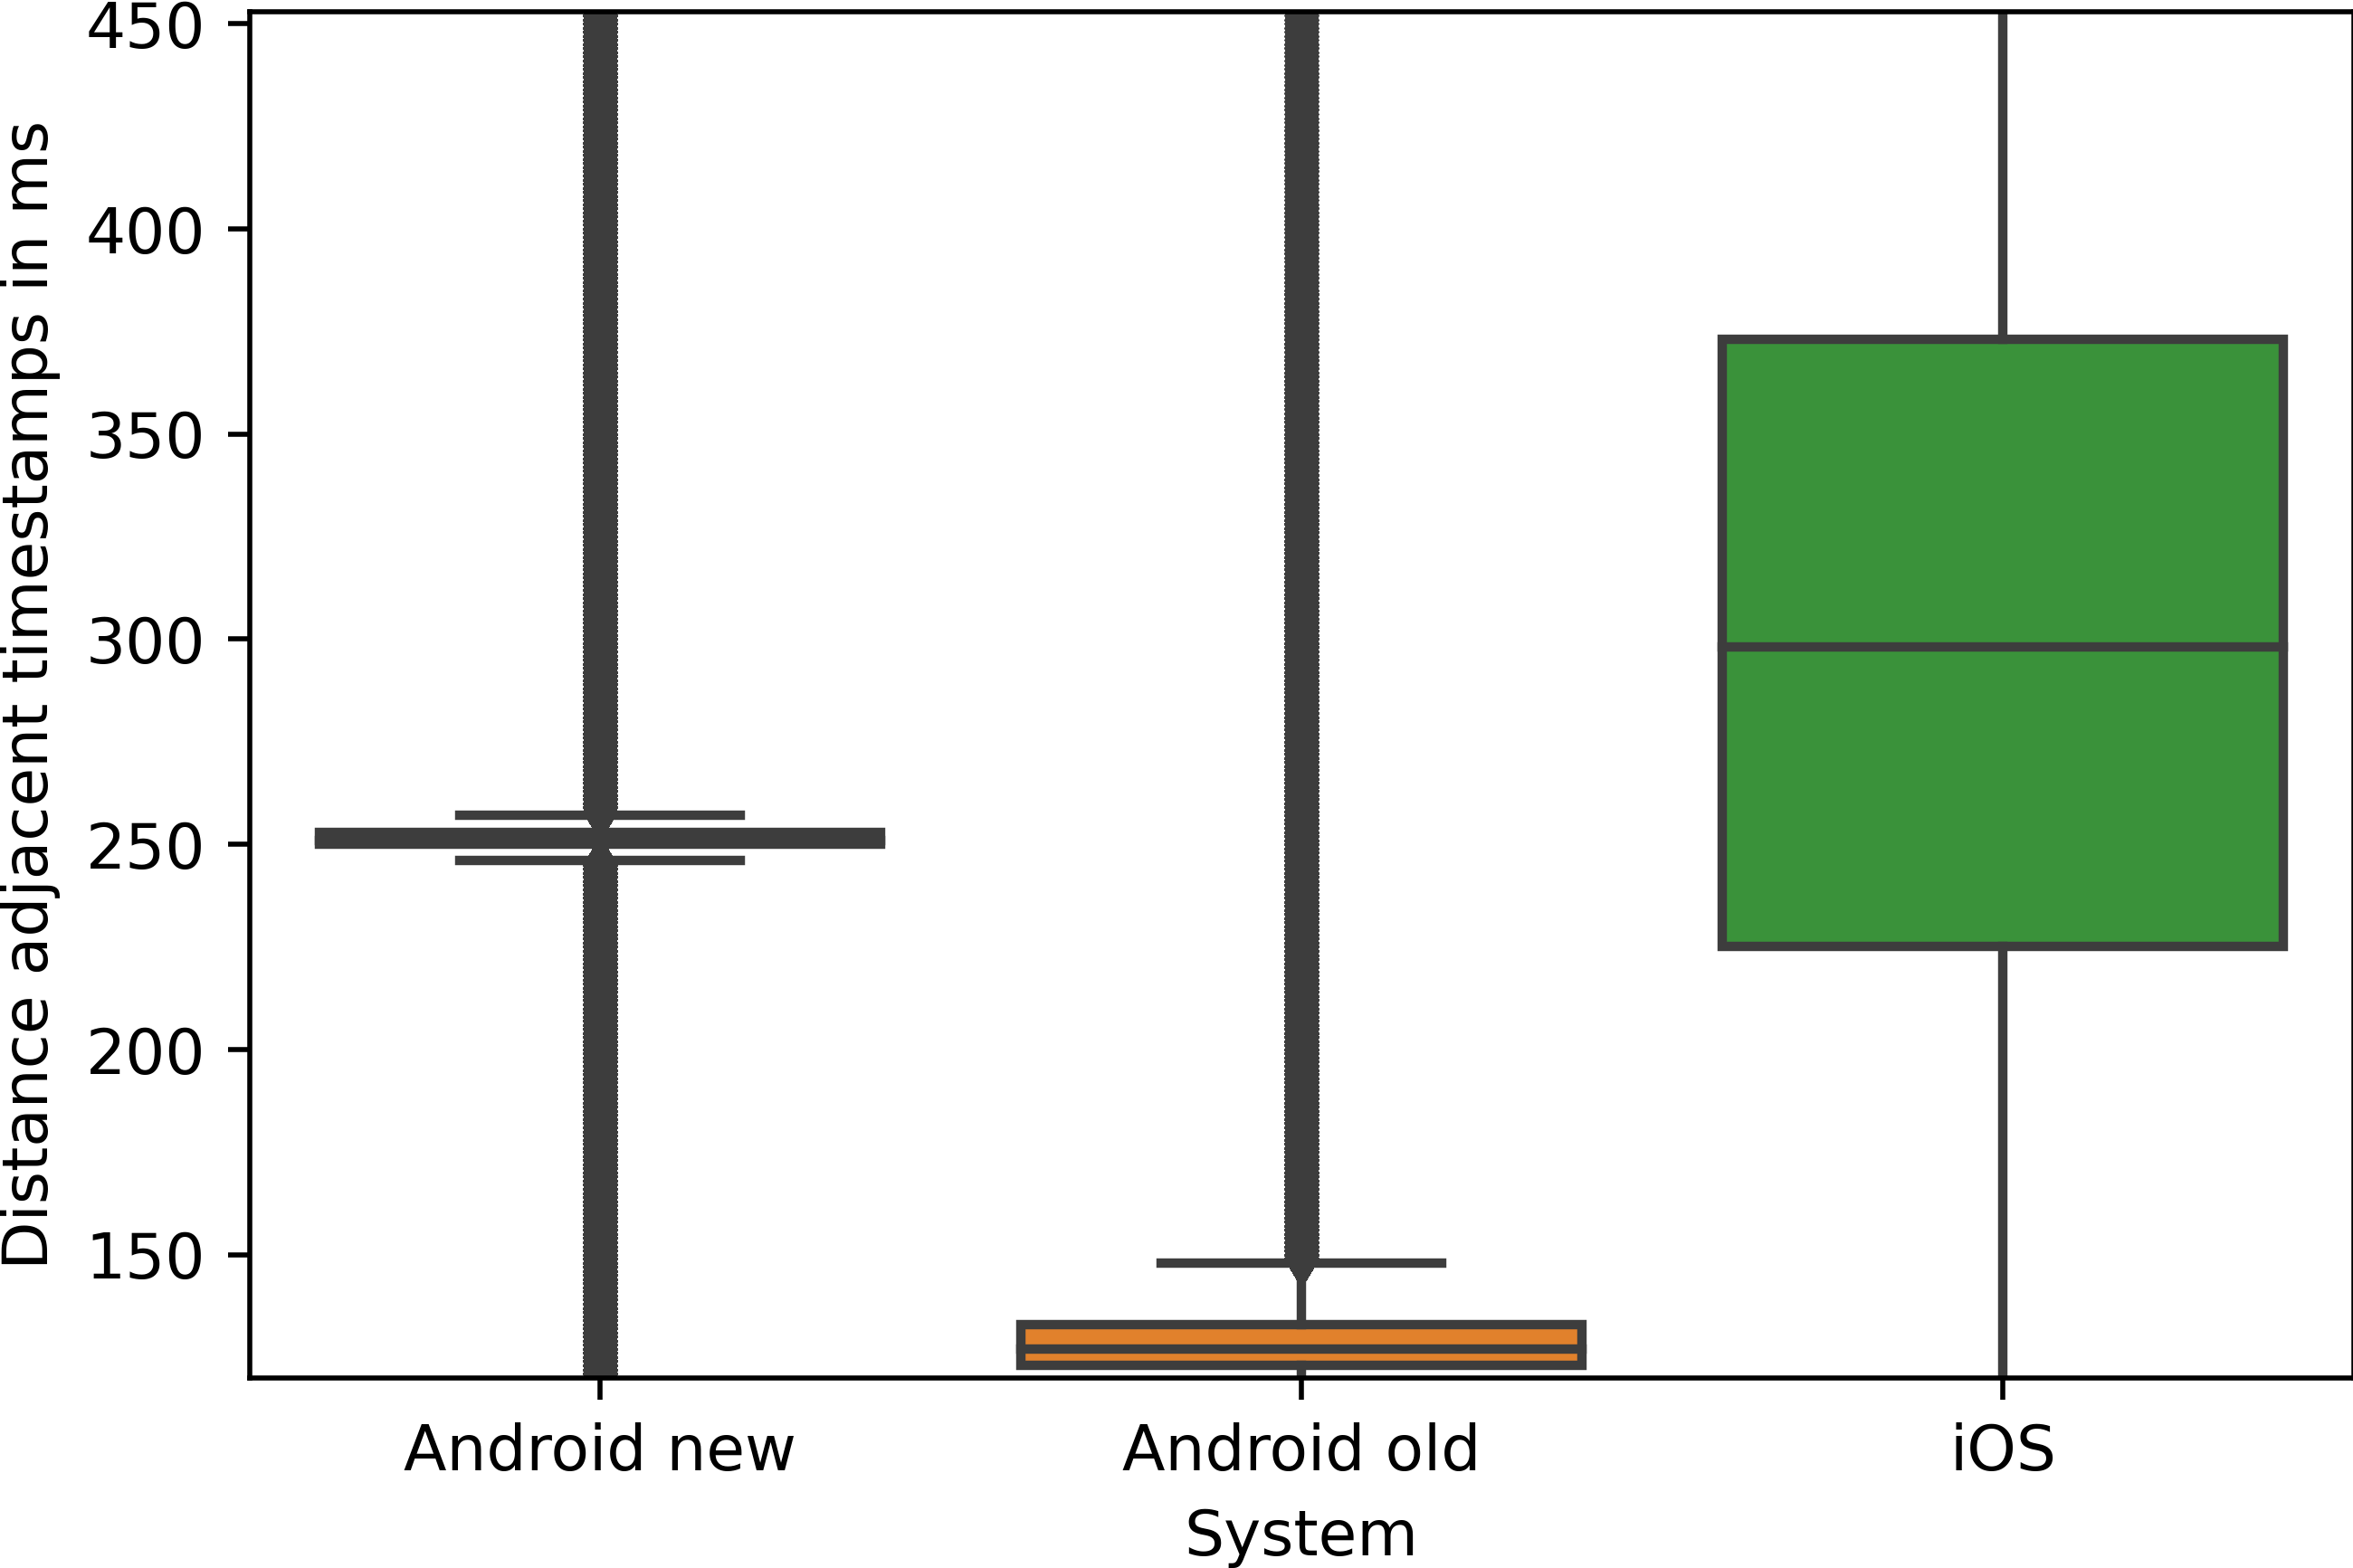
\includegraphics[width=0.45\textwidth]{fig/empirical_measurements.png}
	\caption{Box plot showing the empirical measurement times observed in the SimRa data set for rides recorded with different versions of the SimRa app.}
	\label{fig:emp-measurements}
\end{figure}

Aside from that, the moving average that is used in the SimRa app to condense the data and comply to users' upload volume constraints~\cite{karakaya2020simra} reduces the amplitude and shifts the exact point in time of incidents and other events.
This has the effect that incidents and non-incidents are hard to distinguish as illustrated in Figure~\ref{fig:heavy-vs-normal-braking}.
Both these factors could hurt the model's ability to classify incidents correctly based on the data.
It is important to acknowledge that this issue becomes less severe when the sampling frequency is higher, as it is the case for the older Android data.

\begin{figure}[t]
	\centering
	\begin{subfigure}[b]{0.475\textwidth}
		\centering
		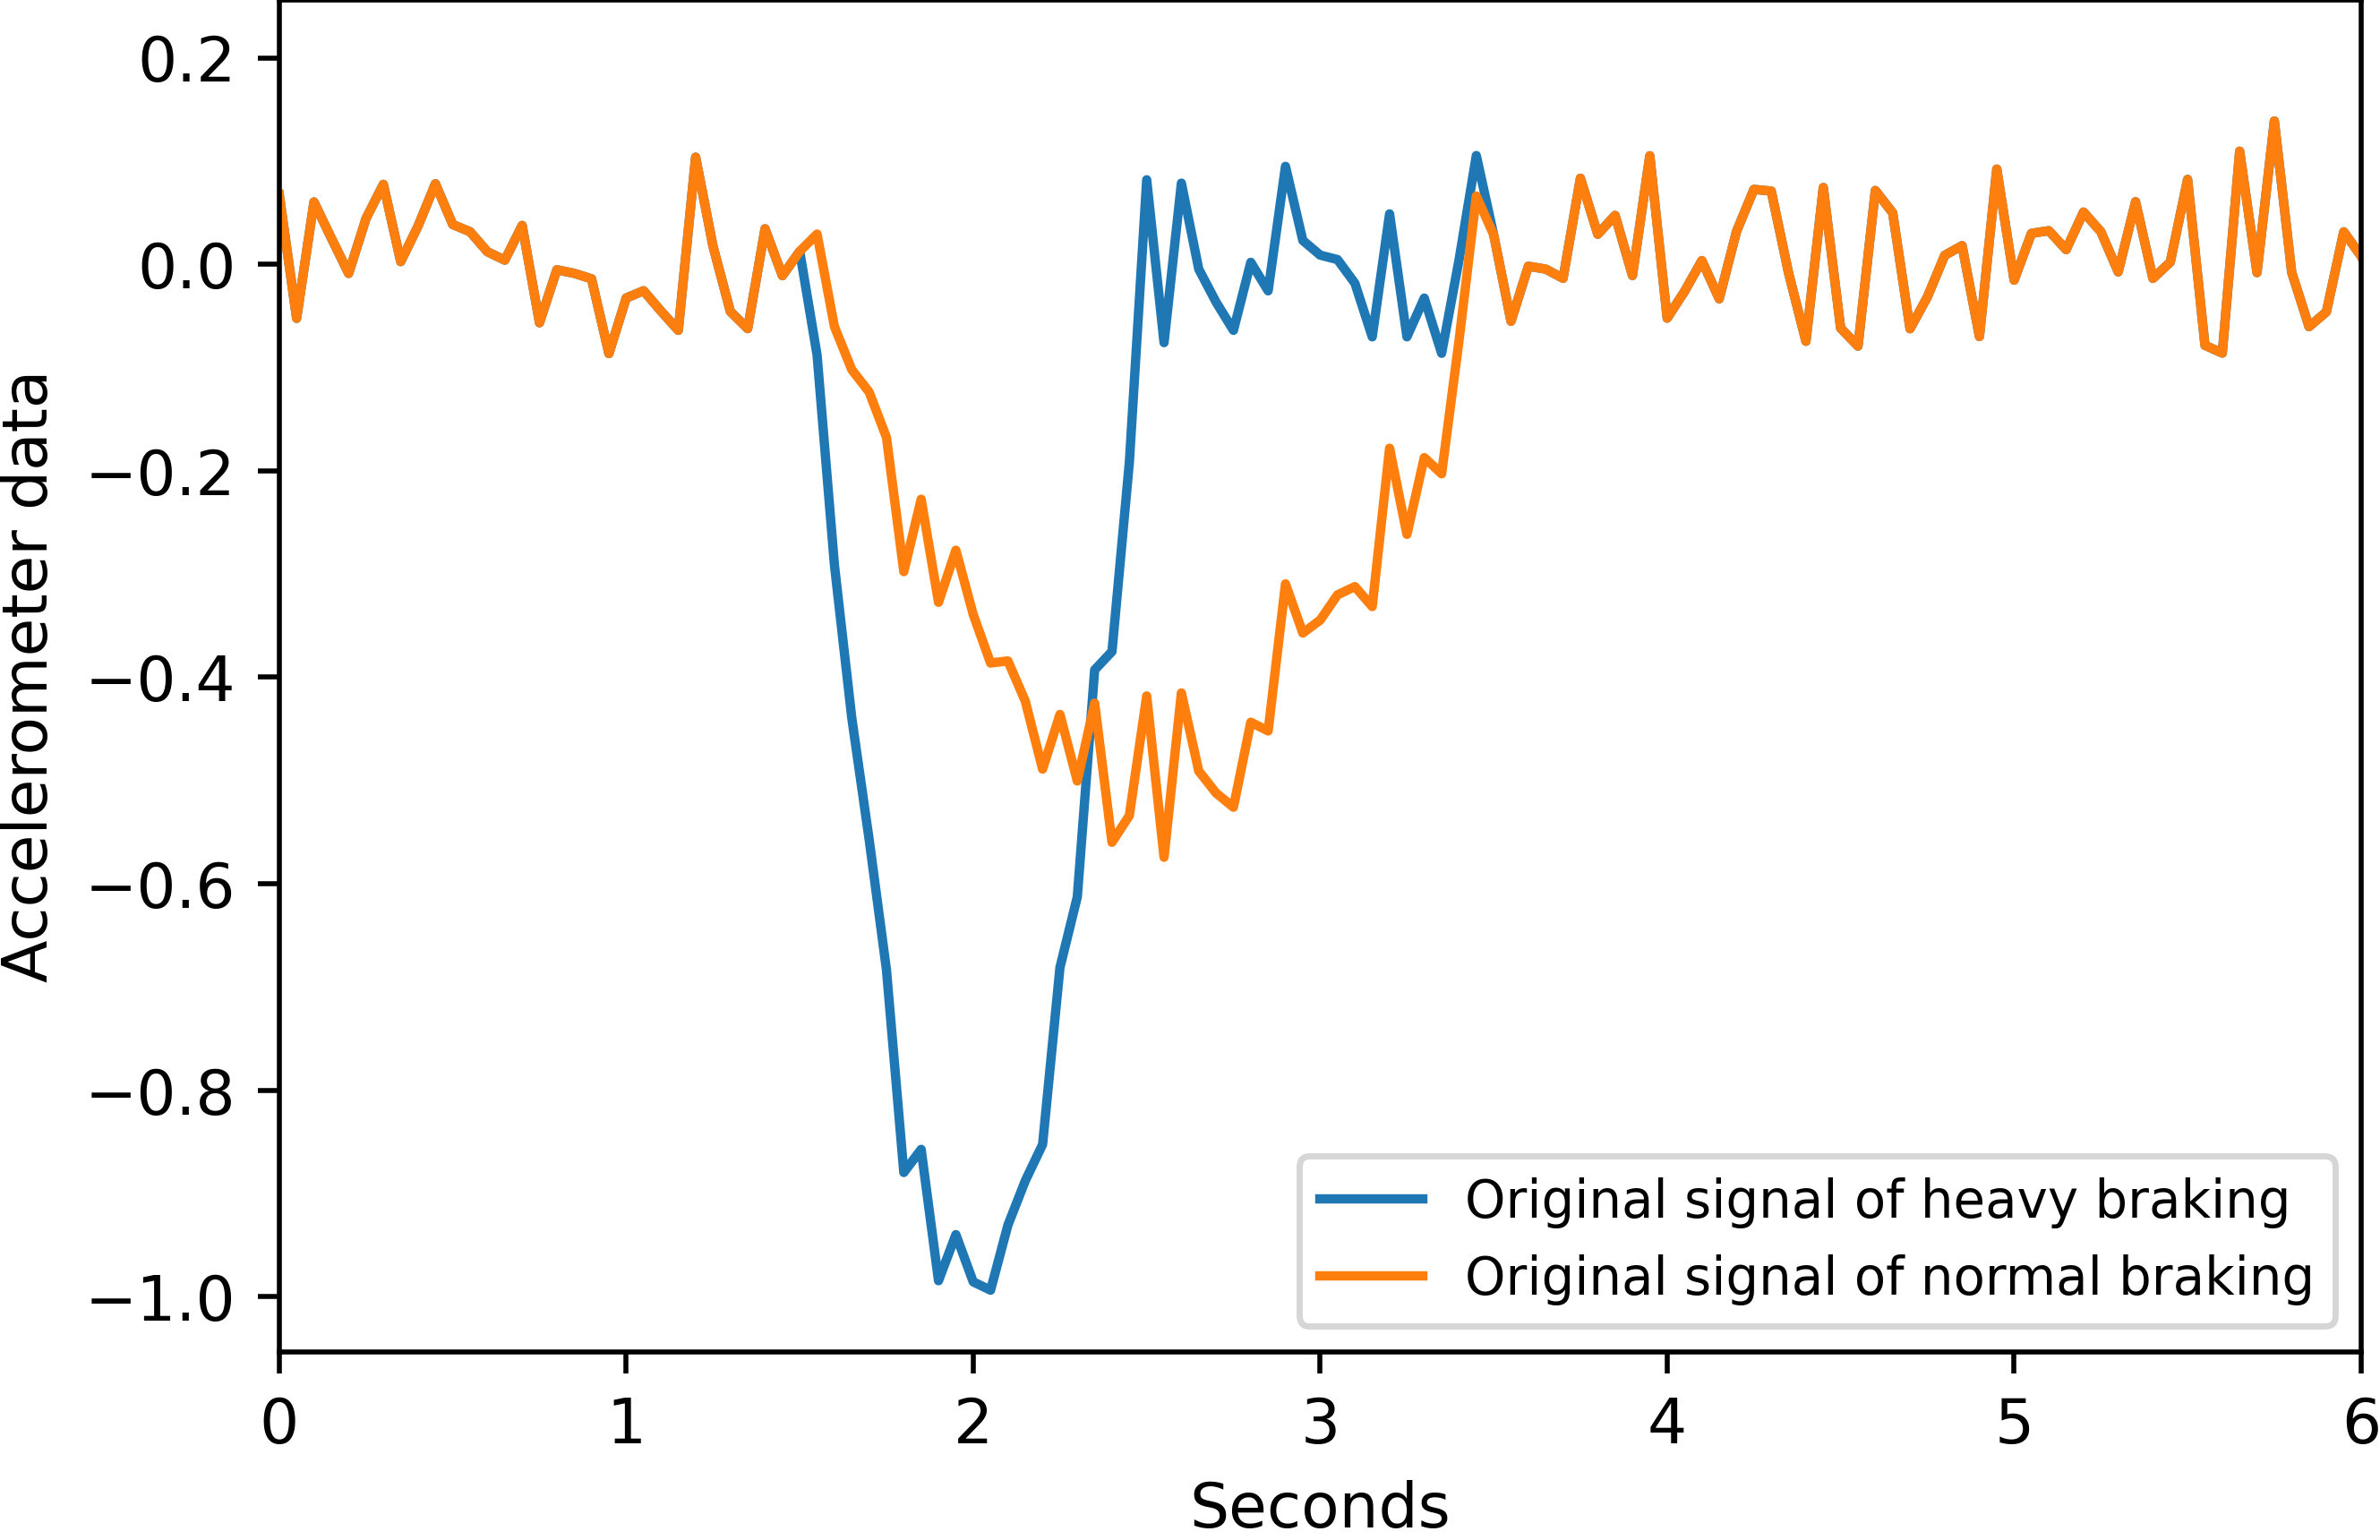
\includegraphics[width=\textwidth]{fig/heavy_vs_normal_braking}
		%\caption{\small Scaled accelerometer data over time of the original signal of an artificially modeled incident with heavy braking vs.\ an artificially modeled moderate braking event.}
	\end{subfigure}
	\hfill
	\begin{subfigure}[b]{0.475\textwidth}
		\centering
		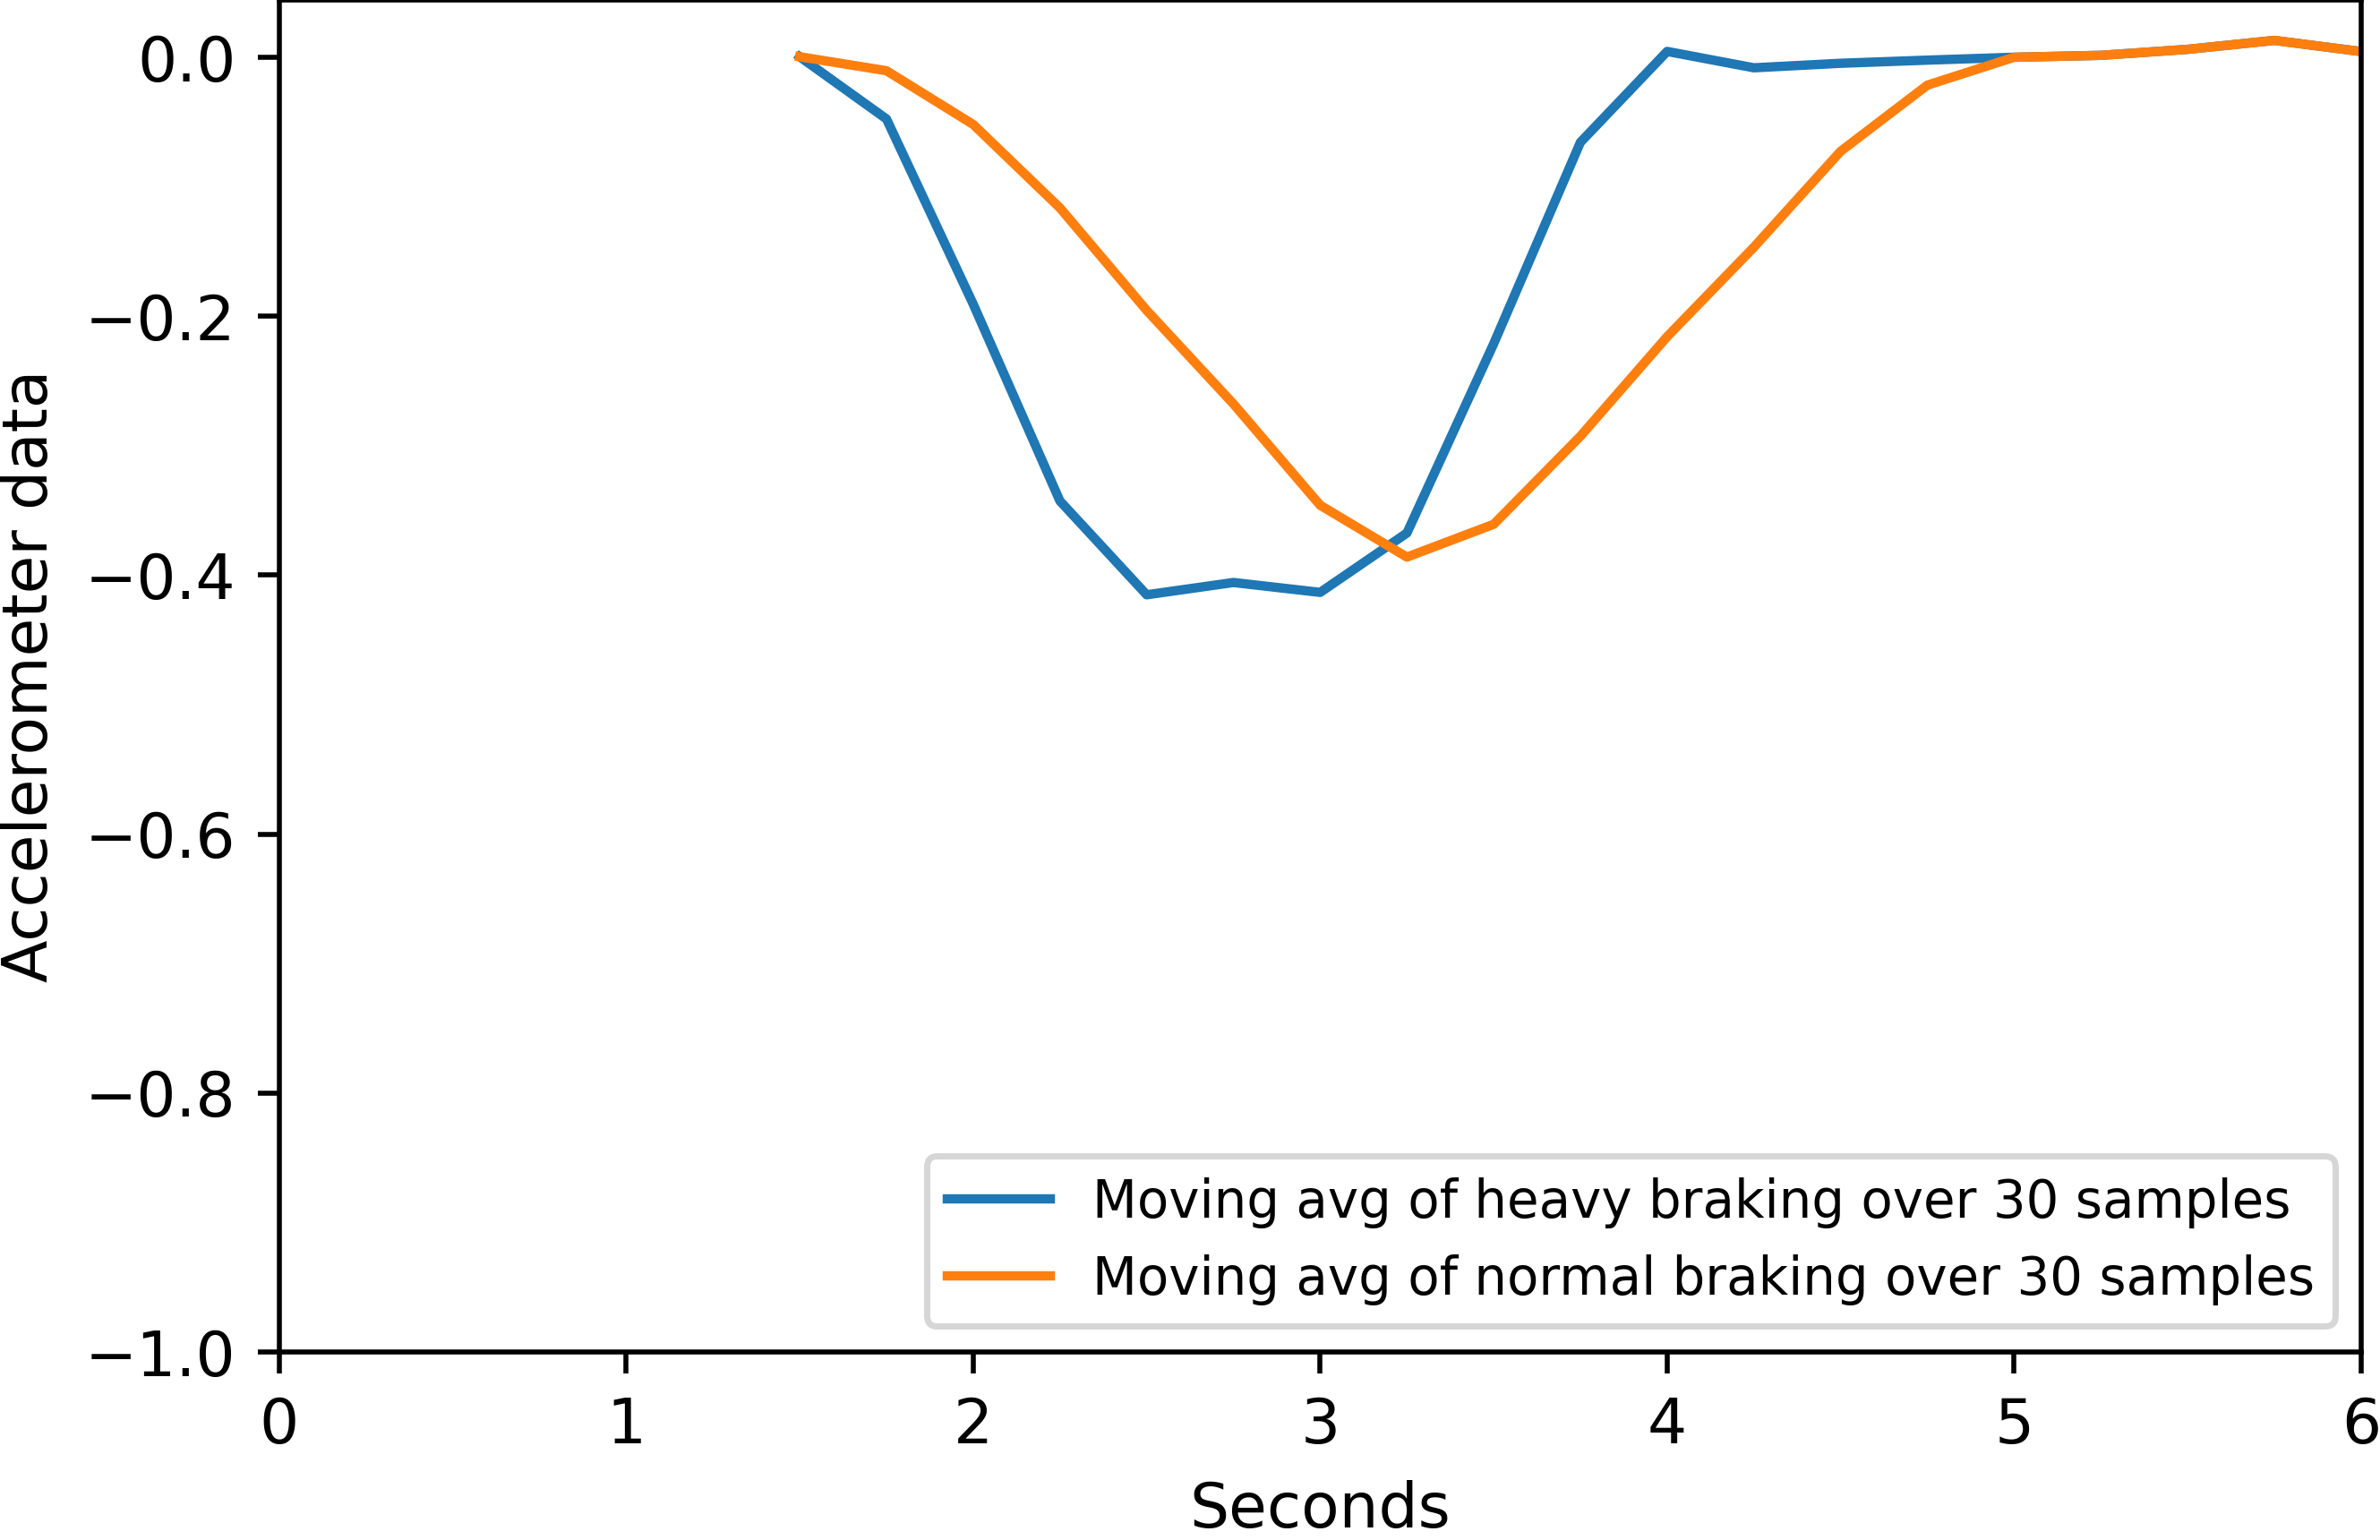
\includegraphics[width=\textwidth]{fig/mvn_avg_heavy_vs_normal_braking.png}
		%\caption{\small Moving average applied on the scaled accelerometer data of the original signal of an artificially modeled incident with heavy braking vs.\ an artificially modeled moderate braking event.}
	\end{subfigure}	
	\caption{Visualization of the sensor data of a simulated heavy braking incident vs.\ a moderate braking event before and after the moving average has been applied.}
	\label{fig:heavy-vs-normal-braking}
\end{figure}

\subsection{Limitation of the Classification Task}
\label{subsec:limitation_of_the_classification_task}
There is an inherent label imbalance present in our data set.
Only relatively few rides contain incidents. 
Moreover, the ratio between timestamps that represent an incident and those that do not is even smaller. 
As a consequence, there is an enormous imbalance between the different label categories.

Furthermore, some incident types such as tailgating or close passes might not be detectable at all in accelerometer and gyroscope sensors~\cite{aldred2018predictors, karakaya2020simra} as cyclists might not change their motion profile despite (or even due to) a dangerous situation.
For detecting these kinds of incidents it may be necessary to include different sensors.
In the SimRa project, this is already happening through an integration of \ac{obs}\footnote{https://www.openbikesensor.org/} data which measures the passing distance of cars.
The current data set, however, only includes very few OBS-supported rides.

In contrast to our classification task, the inherent classification problem of the \ac{har} data set \cite{anguita2013public}, is to classify reoccurring ongoing patterns such as walking or jogging, while an incident might need to be detected by one short non-reoccurring event such as sudden braking.
This further complicates the matter.

\subsection{Data Set Shift}
\label{subsec:data_set_shift}
A major challenge in the context of crowdsourced data are data set shifts.
Depending on the device (see also \autoref{subsec:technical_limitations_of_the_simra_data_set}), but also on other factors, such as the city of origin of the recorded data (see also \autoref{subsec:evaluation_results}), there could be non-stationarities in the data that violate the assumptions underlying almost all ML models and thus could impact the generalization performance of the trained models.
Several types of data set shifts can be distinguished, including \textit{covariate shifts}, meaning shifts in the input data \cite{sugiyama_machine_2012}, \textit{label shifts}, meaning shifts in the distribution of targets \cite{lipton_detecting_2018}, or mixtures thereof.
Detecting these shifts \cite{polyzotis_data_2018, rabanser_failing_2018, breck_data_2019, abdar_review_2021, bates_testing_2021} and predicting \cite{schelter_learning_2020} or reducing their impact on the generalization performance is an active field of research \cite{schelter_challenges_2018, biessmann_automated_2021}.
Some approaches aim at model specific improvements to alleviate data set shift \cite{sugiyama_machine_2012}. These approaches have a decisive disadvantage, most of these approaches only work for one model class and require access to the inner workings of the ML pipeline, often after the feature extraction step.
More promising and easier to build and maintain are model agnostic solutions that focus on the data, rather than the models, to detect and counteract data set shifts \cite{biessmann_automated_2021}.
Extending the training data sets to account for all variation and shifts in the data that the ML model should be invariant to, often called \textit{augmentation}, is a popular and effective way of counteracting data set shift, see for instance \cite{cubuk_autoaugment_2019}.
In our work we follow this line of thought of a data centric AI approach. 


\section{Alternative Approaches}
\label{sec:related_work_cyclesense}
One of the most common tasks for \ac{tsc} are Natural Language Processing, speech recognition, and audio recognition in general.
Another field that deals with this problem is \acf{har} which is concerned with identifying the specific activity of a human based on sensory time series data.
Time windows of a few seconds are classified into activity categories (e.g., walking, sitting, running, lying).
While various feature extraction and pattern recognition methods have been successfully applied in the past in this context~\cite{bulling2014tutorial}, those approaches have constraints such as hand-crafted feature extraction, being able to only learn shallow features~\cite{yang2015deep}, or the requirement for large amounts of well-labeled data for model training~\cite{wang2019deep}.
\acl{dl} techniques and more specifically \acp{cnn} have recently proven to overcome these issues and deliver convincing results in the context of \ac{har}~\cite{wang2019deep,ronao2015deep}.
Also, implementations of \acp{rnn} such as \ac{lstm}~\cite{tao2016multicolumn,yao2017deepsense} have proven to be successful.
Yao et al.\ \cite{yao2017deepsense} use a combination of \acp{rnn} and \acp{cnn} on top of a \ac{sf} approach after preprocessing their input data using a \ac{dft}.

\section{Summary}
\label{sec:summary_cyclesense}
An increased modal share of bicycles is necessary for solving emission and traffic related urban problems.
A key challenge for this, is the lack of (perceived) safety for cyclists.
Improving the situation requires detailed insights into safety levels of street segments -- the SimRa platform~\cite{karakaya2020simra} has been proposed as a data gathering mechanism for incidents and cycling tracks.
While this is an important step towards data collection, the platform relies on manual annotation of tracks which limits the number of potential users.

In this chapter, we have proposed CycleSense -- a model for automatic detection of such incidents.
Using the SimRa data set, we have shown that CycleSense is capable of detecting incidents on the basis of accelerometer and gyroscope time series data in a real-world scenario.
It can correctly distinguish between an incident and a non-incident with a probability of up to 90.5\%.
We have also compared it to the heuristic currently used in the SimRa platform and an existing \ac{fcn} that was specifically developed for SimRa.
Additionally, we have implemented several \ac{dl} models that are frequently used in the context of \ac{tsc}.
We were able to show that our model outperforms all of these approaches.

While this is an important step towards fully automatic incident detection, we believe that -- in the context of the SimRa platform -- CycleSense should be complemented with human annotation in a semi-automated way for the foreseeable future.
Although this does not quite reach our long-term goal of full automation, it should significantly decrease the annotation effort and should also lead to improved labeling quality.
In the future, this could, in turn, be used to further improve CycleSense.
Since April 2022, the SimRa app has been using CycleSense for incident detection.


